% !TeX program = xelatex
\documentclass[a4paper,12pt,oneside]{report}

% Dati del documento e del frontespizio, modificati in un solo posto.
\newcommand{\TitoloTesi}{ChatCart: agente conversazionale con interfaccia generativa}
\newcommand{\AutoreTesi}{Edoardo De Piccoli}
\newcommand{\Matricola}{2101055}
\newcommand{\Relatore}{Prof.\ Tullio Vardanega}
\newcommand{\AnnoAccademico}{2025-2026}

\title{\TitoloTesi}
\author{\AutoreTesi}
\date{}

% Impostazioni comuni: pagina, caratteri, spaziatura e collegamenti.
\usepackage[margin=3cm]{geometry}
\usepackage{fontspec}
\usepackage{lmodern}
\usepackage[italian]{babel}
\usepackage{microtype}
\usepackage{setspace}
\setstretch{1.25}
\usepackage{parskip}
\usepackage{enumitem}
% Elenchi compatti e indivisibili: se non entrano nella pagina passano interi alla successiva.
\makeatletter
\setlist[itemize,enumerate]{nosep, before={\interlinepenalty=10000\relax\@itempenalty=10000\relax}}
\makeatother
\setlength{\emergencystretch}{3em}
% Nessuna riga isolata di un paragrafo in cima o in fondo alla pagina.
% Si impostano a inizio documento perché un pacchetto le riporta a 3000.
\AtBeginDocument{\widowpenalty=10000 \clubpenalty=10000 \displaywidowpenalty=10000}
\setcounter{secnumdepth}{2}
\setcounter{tocdepth}{2}

% Note a piè di pagina sempre in fondo alla pagina, anche quando il testo non la riempie.
\usepackage[bottom]{footmisc}

% Titolo dei capitoli su una riga, con il numero davanti e senza la parola «Capitolo».
\usepackage{titlesec}
\titleformat{\chapter}[hang]{\normalfont\huge\bfseries}{\thechapter}{0.8em}{}
\titlespacing*{\chapter}{0pt}{70pt}{40pt}

\usepackage{graphicx}
\usepackage[table,dvipsnames]{xcolor}

% Diagrammi in TikZ, con gli stessi colori delle tabelle.
\usepackage{tikz}
\usetikzlibrary{arrows.meta,backgrounds,calc,fit,positioning,shapes.geometric}
\definecolor{FiguraTesto}{HTML}{1F2328}
\definecolor{FiguraTenue}{HTML}{59636E}
\definecolor{FiguraBordo}{HTML}{BFBFBF}
\definecolor{FiguraAccento}{HTML}{8C1C2B}
% Seminero di Latin Modern, più stretto del grassetto esteso, per i titoli nei diagrammi.
\newfontfamily\FiguraSeminero{lmromandemi10-regular}[Extension=.otf, ItalicFont=lmromandemi10-oblique]
% Stili comuni: riquadri di raggruppamento con intestazione come nelle tabelle e frecce.
\tikzset{
	partizione/.style={draw=FiguraBordo, fill=TabellaRiga},
	intestazione/.style={draw=FiguraBordo, fill=TabellaIntestazione},
	titolo/.style={font=\footnotesize\bfseries, text=FiguraTesto},
	freccia/.style={draw=FiguraTenue, -{Stealth[length=1.8mm,width=1.4mm]}},
}
% Una voce di diagramma: titolo in seminero e, sotto, un dettaglio più piccolo e grigio.
\newcommand{\voce}[2]{{\fontsize{8.5}{10}\FiguraSeminero #1}\\[2pt]\color{FiguraTenue}#2}
\usepackage{caption}
\captionsetup{font=small}
\usepackage{float}
\floatstyle{plain}
\newfloat{codelisting}{htbp}{lol}[chapter]
\floatname{codelisting}{Codice sorgente}
\usepackage{listings}
\lstset{
	basicstyle=\small\ttfamily,
	breaklines=true,
	columns=fullflexible,
	keepspaces=true,
	showstringspaces=false
}

% Tabelle: stile comune e larghezza complessiva pari al testo.
% Una tabella non si spezza mai tra due pagine: se non entra nello spazio rimasto,
% passa intera alla pagina successiva. Didascalia e identificativo sono argomenti
% dell'ambiente, così la didascalia compare sempre sotto la tabella.
% I margini standard delle colonne allineano sfondi e righe senza patch.
\usepackage{booktabs,array}
\usepackage{needspace}
\definecolor{TabellaIntestazione}{HTML}{E2E5E9}
\definecolor{TabellaRiga}{HTML}{F3F4F6}
\newcolumntype{P}[1]{>{\raggedright\arraybackslash}p{\dimexpr#1\linewidth-2\tabcolsep\relax}}
\newenvironment{tabellatesi}[3]{%
	\def\TabellaDidascalia{#2}%
	\def\TabellaEtichetta{#3}%
	\begin{table}[H]%
	\centering
	\setstretch{1}\fontsize{11}{13.5}\selectfont
	\setlength{\tabcolsep}{8pt}%
	\renewcommand{\arraystretch}{1.3}%
	\setlength{\extrarowheight}{3pt}%
	\setlength{\aboverulesep}{0pt}%
	\setlength{\belowrulesep}{0pt}%
	\arrayrulecolor{black!25}%
	\captionsetup{position=below,skip=6pt}%
	\rowcolors{2}{white}{TabellaRiga}%
	\begin{tabular}{#1}%
}{%
	\end{tabular}%
	\caption{\TabellaDidascalia}\label{\TabellaEtichetta}%
	\end{table}%
}

\usepackage[unicode]{hyperref}
\usepackage{bookmark}
\usepackage{xurl}
\urlstyle{same}
\hypersetup{
	pdftitle={\TitoloTesi},
	pdfauthor={\AutoreTesi},
	pdflang={it-IT},
	colorlinks=true,
	linkcolor=Maroon,
	citecolor=Blue,
	urlcolor=Blue
}

% Riferimenti: il nome e il numero sono un unico collegamento cliccabile.
\newcommand{\figref}[1]{\hyperref[#1]{figura~\ref*{#1}}}
\newcommand{\tabref}[1]{\hyperref[#1]{tabella~\ref*{#1}}}
\newcommand{\secref}[1]{\hyperref[#1]{sezione~\ref*{#1}}}
\newcommand{\codref}[1]{\hyperref[#1]{codice~\ref*{#1}}}
\newcommand{\listoflistings}{\listof{codelisting}{Elenco dei codici sorgente}}

% Capitoli finali senza numero, presenti nell'indice e nei segnalibri PDF.
\newcommand{\capitolononnumerato}[1]{%
	\chapter*{#1}%
	\phantomsection
	\addcontentsline{toc}{chapter}{#1}%
}

% Il pedice G si inserisce esplicitamente solo alla prima occorrenza.
% Termine e pedice fanno parte dello stesso collegamento.
\newcommand{\gloss}[2]{\hyperref[glossario-#1]{#2\textsubscript{G}}}
\newcommand{\rimandoglossario}[2]{\hyperref[glossario-#1]{#2}}
\newcommand{\voceglossario}[3]{%
	\item[\protect\phantomsection\label{glossario-#1}#2] #3%
}


\begin{document}

\hypersetup{pageanchor=false}
% !TeX root = ../tesi.tex

	\begin{titlepage}
		\centering
		{\Large\bfseries Università di Padova\par}
		\vspace{0.8em}
		{\large\textsc{Dipartimento di Matematica “Tullio Levi-Civita”}\par}
		\vspace{0.8em}
		{\large\textsc{Corso di Laurea in Informatica}\par}
		\vfill
		
\includegraphics[width=0.38\textwidth]{figure/comuni/unipd-logo.png}\par
		\vfill
		{\LARGE\bfseries \TitoloTesi\par}
		\vspace{1.2em}
		{\large\scshape Tesi di Laurea\par}
		\vfill
		\begin{minipage}[t]{0.47\textwidth}
			\raggedright
			{\scshape Laureando}\\[0.3em]
			\AutoreTesi\\[0.3em]
			{\scshape Matricola} \Matricola
		\end{minipage}\hfill
		\begin{minipage}[t]{0.47\textwidth}
			\raggedleft
			{\scshape Relatore}\\[0.3em]
			\Relatore
		\end{minipage}
		\vfill
		\rule{0.8\textwidth}{0.4pt}\par
		\vspace{0.6em}
		{\large\textsc{Anno Accademico \AnnoAccademico}\par}
	\end{titlepage}
	\thispagestyle{empty}
	\vspace*{\fill}
	\noindent\small © \AutoreTesi. Tutti i diritti riservati.
	Tesi di Laurea: “\TitoloTesi”, Università di Padova,
	Dipartimento di Matematica “Tullio Levi-Civita”, Corso di Laurea in Informatica.
	\normalsize
	\clearpage


\pagenumbering{roman}
\hypersetup{pageanchor=true}
% !TeX root = ../tesi.tex

\chapter*{Sommario}

In questa relazione descrivo lo \emph{stage} che ho svolto presso Halue S.r.l., società di
consulenza tecnologica con sede operativa ad Abano Terme, dal 14 settembre al 9 novembre 2026.

Con la supervisione del Prof. Tullio Vardanega, relatore, e di Antonio Cavestro, \emph{tutor}
aziendale, ho progettato e realizzato ChatCart, il prototipo di un assistente conversazionale per i
negozi Shopify che risponde al cliente non soltanto con testo, ma anche con componenti
dell’interfaccia che sceglie e popola in tempo reale con i dati del negozio.

\textbf{Struttura del documento.} La relazione si articola in quattro capitoli:

\begin{itemize}
        \item \textbf{Capitolo 1: «Halue e il commercio digitale».} Presento l’azienda, la sua
	clientela, le tecnologie e i processi che adotta e il suo rapporto con l’innovazione, in
	particolare con l’intelligenza artificiale.
        \item \textbf{Capitolo 2: «Oltre la conversazione testuale».} Discuto il problema che lo
	\emph{stage} affronta, il suo posto nella strategia di Halue, gli obiettivi e i vincoli del
	progetto e le ragioni per cui l’ho scelto.
        \item \textbf{Capitolo 3: «Progetto e sviluppo di ChatCart».} Illustro il metodo di lavoro,
	l’analisi, l’architettura, la realizzazione dell’agente e del \emph{widget}, le funzionalità
	sperimentali e le possibili evoluzioni del progetto, la verifica e i risultati ottenuti.
        \item \textbf{Capitolo 4: «Valutazione retrospettiva».} Valuto il grado di soddisfacimento
	degli obiettivi, la mia maturazione professionale e la distanza tra le competenze che lo
	\emph{stage} mi ha richiesto e quelle che ho acquisito nel corso di studi.
\end{itemize}

In appendice raccolgo gli acronimi e le abbreviazioni con la loro forma estesa, il glossario e i riferimenti.

\newpage

\textbf{Convenzioni tipografiche.} Nel documento adotto le seguenti convenzioni:

\begin{itemize}
        \item il corsivo indica i termini in lingua straniera, e soltanto questi; i nomi propri di
	aziende, prodotti e metodi (come Shopify, Slack o Scrum) restano in tondo;
        \item alla prima occorrenza di un termine presente nel glossario ne do nel testo una
	definizione essenziale e lo contrassegno con il pedice G; il termine e il pedice sono cliccabili e
	rimandano all’approfondimento nel glossario;
        \item le figure e le tabelle hanno una numerazione progressiva e una didascalia, che ne
	indica la fonte quando non sono di mia realizzazione.
\end{itemize}

\tableofcontents
\listoffigures
\listoftables
\listoflistings
\clearpage

\pagenumbering{arabic}
% L'ordine dei capitoli è esplicito: i nomi dei file non determinano la compilazione.
% !TeX root = ../tesi.tex

\chapter{Halue e il commercio digitale}

Presento Halue S.r.l., l’azienda presso cui ho svolto lo \emph{stage}, descrivendone le attività, i
clienti, le tecnologie, i processi e il rapporto con l’innovazione. Il quadro nasce dall’esperienza
diretta delle otto settimane di lavoro, dai colloqui con i colleghi, da un’intervista dedicata al
\emph{tutor} aziendale, Antonio Cavestro, e dalle informazioni pubbliche del sito
dell’azienda\textsuperscript{\ref{rif:halue}}.

% !TeX root = ../../tesi.tex

\section{Profilo aziendale e linee di attività}

Halue è una società di consulenza tecnologica nata nel 2022, con sede legale a Parma e sede
operativa ad Abano Terme, in provincia di Padova. È nata come \emph{boutique} di consulenza, cioè
una società piccola e specializzata in pochi ambiti, sull’\gloss{e-commerce}{\emph{e-commerce}} e
sui sistemi di \gloss{crm}{\emph{Customer Relationship Management} (CRM)}, con Shopify e Salesforce
come piattaforme di riferimento. Il primo ambito riguarda la vendita di prodotti e servizi tramite
canali digitali. Il secondo riguarda la gestione delle relazioni delle aziende con i propri
clienti, dalle vendite all’assistenza al \emph{marketing}.

Negli anni successivi Halue ha esteso la propria attività all’intelligenza artificiale, a partire
dai progetti stessi. I negozi dei suoi clienti hanno cataloghi ampi, contenuti in più lingue e
percorsi d’acquisto complessi. In questi punti un modello linguistico collegato ai dati del negozio
aiuta sia chi acquista sia chi gestisce il negozio. Nello stesso periodo le piattaforme di
commercio elettronico hanno iniziato a offrire strumenti e protocolli pensati per gli agenti di
intelligenza artificiale, che presento nella \secref{sec:ecosistema}.

Dal 2024 Halue è una \gloss{societa-benefit}{Società Benefit}: una forma giuridica, introdotta in
Italia nel 2015, per le società che oltre al profitto perseguono obiettivi di beneficio comune
dichiarati nello statuto e ne rendono conto ogni anno in una relazione d’impatto. Gli obiettivi di
Halue riguardano l’ambiente, le persone e le comunità. L’azienda misura le proprie pratiche con il
\gloss{b-impact-assessment}{\emph{B Impact Assessment}}, un questionario di valutazione che le
esamina in cinque aree: \emph{governance}, lavoratori, clienti, comunità e ambiente. Tra i
risultati del 2025, Halue riporta\textsuperscript{\ref{rif:halue-benefit}}:

\begin{itemize}
	\item un codice etico e politiche interne sulla segnalazione di illeciti, sugli abusi e sulle
	discriminazioni;
	\item linee guida per rendere sostenibile il lavoro da remoto;
	\item una collaborazione per la tutela della fauna marina nel Delta del Po.
\end{itemize}

Oggi l’azienda conta dieci persone, con i seguenti ruoli:

\begin{itemize}
        \item \gloss{founder-senior-consultant}{\emph{Founder \& Senior Consultant}}: il fondatore
	Valentino Baraldo, che svolge anche attività di consulenza;
        \item \gloss{solution-technical-architect}{\emph{Solution \& Technical Architect}}:
	definisce le soluzioni e l’architettura tecnica;
        \item \gloss{senior-project-manager}{\emph{Senior Project Manager}} e
	\gloss{project-management-assistant}{\emph{Project Management Assistant}}: due ruoli dedicati alla
	gestione dei progetti;
        \item \gloss{senior-software-engineer}{\emph{Senior Software Engineer}},
	\gloss{software-engineer}{\emph{Software Engineer}} e \gloss{junior-developer}{\emph{Junior
	Developer}}: cinque sviluppatori con diversi livelli di esperienza;
        \item \gloss{ux-ui-digital-consultant}{\emph{UX/UI Digital Consultant}}: cura la
	progettazione dell’esperienza utente e dell’interfaccia.
\end{itemize}

In un’azienda di queste dimensioni ogni ruolo copre un’intera fase del progetto: la consulenza
iniziale, l’architettura, la gestione, lo sviluppo e la progettazione dell’interfaccia. Ogni
persona lavora per più clienti nello stesso periodo.

Halue lavora su commessa: costruisce soluzioni su misura per i singoli clienti e non vende prodotti
propri, come applicazioni pubblicate sullo Shopify App Store. Le sue competenze crescono quindi
progetto dopo progetto, guidate dalle richieste dei clienti, che l’azienda segue da vicino in un
rapporto di lavoro continuo, possibile per un’azienda delle sue dimensioni.

La consulenza tecnologica accompagna tutte le linee di attività dell’azienda, dalla valutazione
iniziale alla scelta dei sistemi. Le linee sono, in ordine di peso:

\begin{enumerate}
        \item l’\emph{e-commerce} su Shopify e su Salesforce Commerce Cloud, sia verso il
	consumatore finale (\gloss{b2c}{B2C}) sia verso altre aziende (\gloss{b2b}{B2B}). Nel B2B il
	negozio gestisce anche listini riservati, ordini minimi e condizioni di pagamento per ciascuna
	azienda cliente;
        \item l’integrazione di sistemi, cioè il collegamento del negozio con la logistica, con i
	servizi di terze parti e con i sistemi gestionali (\gloss{erp}{ERP}), che riuniscono in un’unica
	base di dati amministrazione, acquisti, magazzino e vendite e con cui il negozio sincronizza ordini
	e disponibilità dei prodotti. Il collegamento può essere punto a punto, costruito per ogni coppia di
	sistemi, oppure passare per una piattaforma di integrazione erogata come servizio
	(\gloss{ipaas}{iPaaS}), che offre connettori già pronti e strumenti per trasformare i dati;
        \item i servizi di intelligenza artificiale, dalla valutazione di quanto un’azienda sia
	pronta ad adottarla, anche per la qualità e l’organizzazione dei suoi dati, fino allo sviluppo di
	agenti su misura;
	\item i sistemi CRM su Salesforce, compresi i prodotti per l’assistenza ai clienti e per il
	\emph{marketing};
	\item la formazione, rivolta sia ai clienti sia ai dipendenti. Per i clienti Halue prepara
	incontri come un \emph{workshop} del fondatore sul funzionamento dei modelli linguistici, che
	aggiorna il cliente su questa tecnologia e lo rende consapevole delle sue possibilità e dei suoi
	limiti. I dipendenti seguono una formazione interna sui metodi agili, sulle piattaforme e sulla
	tecnologia, e percorsi personali come il corso di \emph{project management} che un collega
	seguiva durante il mio \emph{stage}: si formano per crescere come professionisti, anche oltre il
	loro ruolo in azienda;
	\item la progettazione dell’interfaccia e dell’esperienza utente.
\end{enumerate}

Le due piattaforme di \emph{e-commerce} hanno pesato in modo diverso nella storia di Halue. Nei
primi anni l’azienda si è specializzata anche su Salesforce Commerce Cloud, la piattaforma di
commercio elettronico della \emph{suite} di Salesforce, e ne segue ancora i clienti. Oggi la
specializzazione principale è Shopify Plus, che presento nella \secref{sec:clientela}. Halue cura
anche la migrazione completa di un negozio da una piattaforma all’altra.

L’intelligenza artificiale è insieme una linea a sé e, sempre di più, una competenza che entra
nei progetti di \emph{e-commerce} e di integrazione.


% !TeX root = ../../tesi.tex

\section{Clientela e modalità di ingaggio}
\label{sec:clientela}

Halue lavora soltanto con aziende private, per lo più di medie e grandi dimensioni, e non con la
pubblica amministrazione. Sono marchi strutturati della moda, dello sport, del commercio al
dettaglio e della cosmetica professionale, con fatturati che vanno da decine a diverse centinaia di
milioni di euro all’anno, e vendono \emph{online} su più mercati, con lingue e valute diverse. La
maggior parte dei clienti è italiana, ma ci sono anche marchi esteri.

Vendere su più mercati moltiplica il lavoro tecnico. Ogni mercato ha la sua lingua, la sua valuta,
i suoi prezzi e le sue tasse, spesso anche un magazzino proprio, e ogni negozio deve restare
allineato con il sistema gestionale dell’azienda. Per questo molti clienti di Halue usano
\gloss{shopify-plus}{Shopify Plus}, la proposta di Shopify per le aziende di grandi dimensioni, che
aggiunge al negozio, tra l’altro, funzioni dedicate alla vendita
B2B\textsuperscript{\ref{rif:shopify-plus}}. Alcuni clienti hanno decine di negozi attivi, uno per
mercato o per canale, ciascuno con il proprio catalogo e il proprio magazzino.

Halue è \emph{Shopify Plus Partner} dal 2023. Il programma partner di Shopify assegna alle agenzie
un livello in base ai negozi che hanno avviato o trasferito sulla piattaforma e al volume di vendite
di quei negozi. Il livello dà all’agenzia visibilità nell’elenco ufficiale dei partner, che i
commercianti consultano per scegliere a chi affidare il proprio negozio. Nel suo profilo Halue
indica come specializzazioni, tra le altre, lo sviluppo di applicazioni e API su misura, la
personalizzazione del processo di pagamento e degli account dei clienti e l’ottimizzazione per i
motori di ricerca\textsuperscript{\ref{rif:halue-partner}}.

Le richieste dei clienti rientrano in quattro tipi:

\begin{itemize}
	\item la migrazione di un negozio verso Shopify da altre piattaforme, come Salesforce Commerce
	Cloud, WooCommerce e Magento. Oltre a catalogo, clienti e ordini, la migrazione trasferisce le
	integrazioni con i sistemi esterni e conserva gli indirizzi delle pagine, perché i collegamenti
	esistenti e il posizionamento nei motori di ricerca non vadano persi;
	\item il \gloss{redesign}{\emph{redesign}} di un negozio esistente;
	\item lo sviluppo di interfacce su misura, con \gloss{landing-page}{\emph{landing page}}
	dinamiche e configuratori 3D;
	\item l’espansione su nuovi mercati e la manutenzione periodica dei negozi in produzione, con
	aggiornamenti di configurazione, correzioni ed evoluzioni.
\end{itemize}

Durante il mio \emph{stage} le manutenzioni e gli aggiornamenti erano il tema più frequente nelle
riunioni quotidiane del \emph{team}.

I progetti arrivano soprattutto per passaparola, da clienti e contatti che segnalano l’azienda, e
in parte da gare e bandi. Le formule contrattuali sono tre, ciascuna adatta a un tipo di lavoro:

\begin{itemize}
	\item a corpo, con un prezzo fissato in anticipo, per i progetti dal perimetro ben definito.
	Questa formula richiede una stima accurata prima di iniziare, e nella
	\secref{sec:ciclo-ticket} descrivo il metodo con cui Halue la ottiene;
	\item a tempo e materiali, per i lavori il cui perimetro si chiarisce strada facendo. Il
	cliente paga il tempo impiegato, calcolato sul costo giornaliero di ciascun dipendente
	moltiplicato per il numero dei dipendenti coinvolti e per le giornate di lavoro;
	\item i contratti di manutenzione e assistenza per i negozi già in produzione, che coprono le
	segnalazioni e le evoluzioni dopo la consegna.
\end{itemize}

Le modifiche chieste a progetto avviato diventano \emph{change request} e seguono lo stesso
percorso di stima del progetto iniziale. Il rapporto con un cliente prosegue quindi oltre la
consegna, e con alcuni clienti è diventato una collaborazione duratura, comprensiva di più progetti
successivi alla prima collaborazione con l’azienda.

Il fondatore e il \emph{Senior Project Manager} sono le figure che seguono i clienti con più
continuità. Quando un cliente collabora da tempo con uno sviluppatore, per esempio un \emph{Senior
Software Engineer}, le richieste di nuove funzionalità e gli aggiornamenti sull’avanzamento passano
direttamente da quella persona, nelle \emph{call} e nel canale Slack dedicato al marchio.


% !TeX root = ../../tesi.tex

\section{Ecosistema tecnologico}
\label{sec:ecosistema}

Le interfacce dei negozi Shopify rivolte ai clienti, dette \gloss{storefront}{\emph{storefront}}, si
possono sviluppare in due modi:

\begin{itemize}
        \item con un tema della piattaforma: Shopify genera le pagine a partire da modelli scritti in
	\gloss{liquid}{Liquid}, il suo linguaggio di \emph{templating}, e dai dati del negozio;
        \item con un’architettura \gloss{headless}{\emph{headless}}: l’interfaccia è un’applicazione
	separata, costruita per esempio con \gloss{hydrogen}{Hydrogen}, il \emph{framework} di Shopify
	basato su React, e accede al negozio tramite \gloss{api}{API}, cioè interfacce con cui un
	programma mette a disposizione di altri programmi dati e operazioni, secondo un contratto definito.
\end{itemize}

Shopify offre due famiglie di API: le Admin API, per gestire i dati e le operazioni del negozio, e
le Storefront API, per catalogo, carrello e acquisto. Entrambe usano \gloss{graphql}{GraphQL}, un
linguaggio di interrogazione in cui il \emph{client} chiede con una sola richiesta esattamente i
campi che gli servono. Un tema Liquid riceve invece i dati del negozio durante la generazione delle
pagine. Per aggiungere funzionalità, Halue sviluppa applicazioni personalizzate in Node.js e
TypeScript, integrabili con entrambe le modalità.

Nei progetti di intelligenza artificiale cambia soprattutto l’architettura. Al centro c’è un
\gloss{llm}{modello linguistico di grandi dimensioni (LLM)}, addestrato a elaborare e generare
testo, che chiede all’agente che lo ospita di invocare uno strumento, ne riceve il risultato e
ripete il ciclo finché non formula la risposta (\figref{fig:agente}). Gli strumenti si possono
scrivere su misura per il progetto oppure ottenere tramite \gloss{mcp}{MCP}, un protocollo aperto
con cui un \emph{server} espone strumenti e risorse, come il catalogo di un negozio, a qualunque
agente lo supporti, senza un’integrazione dedicata per ciascuno.

In ChatCart ho sviluppato una ricerca nel catalogo su misura al posto del \emph{server} MCP di
Shopify: da questa scelta nasce il contratto tra agente e \emph{widget} che descrivo nella
\secref{sec:contratto}.

\begin{figure}[htbp]
	\centering
	\setstretch{1}
	% L'architettura di un progetto di intelligenza artificiale in Halue: l'applicazione dell'agente
% sta tra l'utente, il modello e i servizi esterni da cui arrivano dati e azioni.
% In bordeaux le parti sviluppate per ogni progetto.
% Il disegno è largo quanto il testo (150 mm): si include con \input, senza ridimensionarlo.

\begin{tikzpicture}[
	every node/.style={text=FiguraTesto},
	blocco/.style={draw=FiguraTenue, fill=white, rounded corners=3pt, text width=#1-2mm,
		minimum width=#1, minimum height=11mm, align=center, inner sep=1.5pt,
		font=\fontsize{7.5}{9}\selectfont,
		execute at begin node={\hyphenpenalty=10000\exhyphenpenalty=10000}},
	blocco/.default=40mm,
	interno/.style={draw=FiguraAccento, line width=0.8pt},
	doppia/.style={freccia, {Stealth[length=1.8mm,width=1.4mm]}-{Stealth[length=1.8mm,width=1.4mm]}},
	etichetta/.style={font=\fontsize{7.5}{9}\selectfont, text=FiguraTenue, inner sep=1pt,
		align=center},
]
	% L'applicazione dell'agente e i servizi esterni, come contenitori sullo sfondo.
	\begin{scope}[on background layer]
		\path[partizione] (32mm, -24mm) rectangle (98mm, -76mm);
		\path[intestazione] (32mm, -24mm) rectangle (98mm, -30mm);
		\node[titolo] at (65mm, -27mm) {Applicazione dell’agente};
		\path[partizione] (106mm, -24mm) rectangle (150mm, -76mm);
		\path[intestazione] (106mm, -24mm) rectangle (150mm, -30mm);
		\node[titolo] at (128mm, -27mm) {Servizi esterni};
	\end{scope}

	% Il modello, fuori dall'applicazione che lo usa.
	\node[blocco=66mm] (llm) at (65mm, -6.5mm)
		{\voce{Modello linguistico (LLM)}{servizio del fornitore, di solito Claude}};

	% Dentro l'applicazione.
	\node[blocco=54mm, interno] (istruzioni) at (65mm, -38.5mm)
		{\voce{Istruzioni}{compito, regole, tono del marchio}};
	\node[blocco=54mm, interno] (strumenti) at (65mm, -52.5mm)
		{\voce{Strumenti interni}{ricerche e azioni su misura del progetto}};
	\node[blocco=54mm] (client) at (65mm, -66.5mm)
		{\voce{\emph{Client} MCP}{scopre e invoca gli strumenti dei \emph{server}}};

	% Fuori dall'applicazione.
	\node[blocco=22mm, minimum height=16mm] (utente) at (11mm, -52.5mm)
		{\voce{Utente}{scrive in linguaggio naturale}};
	\node[blocco=40mm] (ucp) at (128mm, -38.5mm)
		{\voce{Negozio con UCP}{carrello, \emph{checkout}, pagamento}};
	\node[blocco=40mm] (api) at (128mm, -52.5mm)
		{\voce{API della piattaforma}{Shopify, Salesforce, gestionali}};
	\node[blocco=40mm] (mcp) at (128mm, -66.5mm)
		{\voce{\emph{Server} MCP}{della piattaforma o di terze parti}};

	% Il ciclo tra applicazione e modello.
	\draw[freccia] (58mm, -24mm) -- (58mm, -12mm);
	\draw[freccia] (72mm, -12mm) -- (72mm, -24mm);
	\node[etichetta, anchor=east] at (56.5mm, -18mm) {conversazione, istruzioni,\\descrizione degli strumenti};
	\node[etichetta, anchor=west] at (73.5mm, -18mm) {testo, oppure\\strumento da invocare};

	% Collegamenti con l'esterno.
	\draw[doppia] (utente.east) -- (32mm, -52.5mm);
	\draw[freccia] (strumenti.east) -- (api.west);
	\draw[freccia] (102mm, -52.5mm) |- (ucp.west);
	\fill[FiguraTenue] (102mm, -52.5mm) circle (0.5mm);
	\draw[freccia] (client.east) -- (mcp.west);
\end{tikzpicture}

	\caption{Esempio di architettura di un progetto di intelligenza artificiale.}
	\label{fig:agente}
\end{figure}


% !TeX root = ../../tesi.tex

\section{Processi di sviluppo e gestione dei progetti}

\subsection{Organizzazione del lavoro e gestione dei progetti}
\label{sec:organizzazione-halue}

Il metodo di riferimento è \gloss{scrum}{Scrum}, un \emph{framework} agile per lo sviluppo
iterativo, adattato al lavoro di un’agenzia. Il lavoro procede per \gloss{sprint}{\emph{sprint}},
cicli brevi al termine dei quali il \emph{team} presenta i risultati al cliente in una \emph{sprint
review} e ne discute internamente in una retrospettiva. Mancano le figure canoniche di Scrum, il
\emph{Product Owner} e lo \emph{Scrum Master}, e le loro responsabilità passano a due ruoli:

\begin{itemize}
	\item il \gloss{team-lead}{\emph{team lead}}, che cura l’analisi funzionale, le stime per il
	cliente e il coordinamento tecnico;
	\item il \gloss{project-service-manager}{\emph{project/service manager}}, che pianifica le
	attività e la capacità del \emph{team}.
\end{itemize}

Accanto a loro lavorano gli sviluppatori e chi progetta l’interfaccia. In un’agenzia lo stesso
gruppo di persone lavora per più clienti nello stesso periodo, perciò nessuno è assegnato a un
progetto in modo stabile: ogni mese un \emph{demand planning} condiviso ripartisce il \emph{team}
sui clienti, e un rapporto sullo \gloss{sal}{stato di avanzamento dei lavori (SAL)} riporta con un
semaforo lo stato di ciascun progetto, le scadenze, i rischi e i punti aperti.

Il \emph{team} si coordina con gli strumenti della \tabref{tbl:coordinamento} e con uno
\gloss{stand-up}{\emph{stand-up}} quotidiano, una riunione mattutina di quindici-venti minuti in
cui ciascuno espone su cosa ha lavorato il giorno prima e su cosa lavorerà quel giorno.

\begin{tabellatesi}{P{0.3}P{0.7}}
	{Gli strumenti di coordinamento del \emph{team} di Halue.}
	{tbl:coordinamento}
	\toprule
	\rowcolor{TabellaIntestazione} \textbf{Strumento} & \textbf{Uso} \\
	\midrule
	Google Meet & riunioni a distanza, tra cui lo \emph{stand-up} \\
	Jira & registro delle richieste e \emph{board} di avanzamento dei progetti \\
	Slack & comunicazione con i clienti, in un canale per ciascun marchio \\
	\emph{Email} & resoconti delle attività e variazioni contrattuali \\
	Confluence e Google Drive & documentazione e conoscenza interna \\
	\bottomrule
\end{tabellatesi}

Gli orari e il luogo di lavoro sono flessibili: i dipendenti lavorano in sede indicativamente tra
il 30\% e il 40\% del tempo e da remoto per il resto, e ognuno gestisce la propria presenza in
autonomia. L’inserimento di un nuovo membro del \emph{team} parte dalla documentazione e dalle
procedure interne e prosegue con piccoli \gloss{ticket}{\emph{ticket}}, le unità di lavoro che Jira
registra con un identificativo, una descrizione e uno stato, su un progetto reale e con
l’affiancamento di un collega.

\subsection{Dal \emph{ticket} al rilascio}
\label{sec:ciclo-ticket}

La \figref{fig:ticket} mostra il percorso di una richiesta del cliente, dal \emph{ticket} su Jira
alla manutenzione.

\begin{figure}[htbp]
	\centering
	\setstretch{1}
	% Il ciclo di vita di un ticket in Halue, come diagramma di attività UML.
% Le partizioni sono le tre fasi; il flusso va da sinistra a destra su due righe.
% Il disegno è largo quanto il testo (150 mm): si include con \input, senza ridimensionarlo.

\begin{tikzpicture}[
	every node/.style={text=FiguraTesto},
	azione/.style={draw=FiguraTenue, fill=white, rounded corners=3pt, text width=18.7mm,
		minimum width=19.8mm, minimum height=15mm, align=center, inner sep=1.5pt,
		font=\fontsize{7.5}{9}\selectfont,
		execute at begin node={\hyphenpenalty=10000\exhyphenpenalty=10000}},
	decisione/.style={draw=FiguraTenue, fill=white, diamond, minimum size=6mm, inner sep=0pt},
	iniziale/.style={circle, fill=FiguraTesto, minimum size=3mm, inner sep=0pt},
	finale/.style={circle, draw=FiguraTesto, fill=white, minimum size=3.6mm, inner sep=0pt,
		path picture={\fill[FiguraTesto] (path picture bounding box.center) circle (1.05mm);}},
	flusso/.style={freccia},
	guardia/.style={font=\fontsize{7.5}{9}\selectfont, text=FiguraTenue, inner sep=1pt},
	node distance=4mm,
]
	% Prima riga: analisi.
	\node[iniziale] (inizio) at (4mm, -20mm) {};
	\node[azione, right=of inizio] (richiesta)
		{\voce{Richiesta}{del cliente per \emph{call}, \emph{email} o \emph{workshop}}};
	\node[azione, right=of richiesta] (ticket)
		{\voce{\emph{Ticket} su Jira}{\emph{Epic}, \emph{Story}, \emph{Change Request} o \emph{Bug}}};
	\node[azione, right=of ticket] (funzionale)
		{\voce{\emph{Refinement} funzionale}{completezza e fattibilità}};
	\node[decisione, right=of funzionale] (bug) {};
	\node[azione, right=7mm of bug] (tecnico)
		{\voce{\emph{Refinement} tecnico}{svolto dagli sviluppatori}};
	\node[decisione, right=of tecnico] (unione) {};
	\node[azione, right=of unione] (stima)
		{\voce{Stima}{\emph{story point} per il \emph{team}, ore per il cliente}};

	% Seconda riga: sviluppo, verifica e rilascio.
	\node[azione] (branch) at (12.4mm, -52mm)
		{\voce{Sviluppo}{su un \emph{branch} con la chiave del \emph{ticket}}};
	\node[azione, right=3.5mm of branch] (pr)
		{\voce{\emph{Pull request}}{\emph{test} automatici e manuali}};
	\node[azione, right=3.5mm of pr] (designer)
		{\voce{Revisione}{del \emph{designer} prima del rilascio}};
	\node[azione, right=5mm of designer] (collaudo)
		{\voce{Collaudo}{del cliente in \emph{staging}}};
	\node[azione, right=3.5mm of collaudo] (produzione)
		{\voce{Rilascio in produzione}{\emph{deploy} avviato a mano}};
	\node[azione, right=3.5mm of produzione] (manutenzione)
		{\voce{Manutenzione}{le segnalazioni diventano nuovi \emph{ticket}}};
	\node[finale, right=3.5mm of manutenzione] (fine) {};

	% Riferimenti per partizioni e percorsi a gomito.
	\coordinate (scavalco) at (0, -9.5mm);
	\coordinate (ritorno) at (0, -33mm);
	\coordinate (riga2) at (0, -36mm);
	\coordinate (fondo2) at (0, -62mm);
	\coordinate (confine) at ($(designer.east)!0.5!(collaudo.west)$);
	\coordinate (confine-alto) at (confine |- riga2);
	\coordinate (confine-basso) at (confine |- fondo2);

	% Partizioni, sullo sfondo, con l'intestazione nello stile delle tabelle.
	\begin{scope}[on background layer]
		\path[partizione] (0, 0) rectangle (150mm, -30mm);
		\path[intestazione] (0, 0) rectangle (150mm, -6mm);
		\node[titolo] at (75mm, -3mm) {Analisi};
		\path[partizione] (riga2) rectangle (confine-basso);
		\path[intestazione] (riga2) rectangle ($(confine-alto) + (0, -6mm)$);
		\node[titolo] at ($(riga2)!0.5!(confine-alto) + (0, -3mm)$) {Sviluppo};
		\path[partizione] (confine-alto) rectangle (150mm, -62mm);
		\path[intestazione] (confine-alto) rectangle (150mm, -42mm);
		\node[titolo] at ($(confine-alto)!0.5!(150mm, -36mm) + (0, -3mm)$) {Verifica e rilascio};
	\end{scope}

	% Flusso di controllo.
	\draw[flusso] (inizio) -- (richiesta);
	\draw[flusso] (richiesta) -- (ticket);
	\draw[flusso] (ticket) -- (funzionale);
	\draw[flusso] (funzionale) -- (bug);
	\draw[flusso] (bug) -- node[guardia, above] {[no]} (tecnico);
	\draw[flusso] (bug.north) -- (bug.north |- scavalco)
		-- node[guardia, above] {[sì]} (unione.north |- scavalco) -- (unione.north);
	\draw[flusso] (tecnico) -- (unione);
	\draw[flusso] (unione) -- (stima);
	\node[guardia, below=1mm of bug] {È un \emph{bug}?};
	\draw[flusso] (stima.south) -- (stima.south |- ritorno) -- (branch.north |- ritorno)
		-- (branch.north);
	\draw[flusso] (branch) -- (pr);
	\draw[flusso] (pr) -- (designer);
	\draw[flusso] (designer) -- (collaudo);
	\draw[flusso] (collaudo) -- (produzione);
	\draw[flusso] (produzione) -- (manutenzione);
	\draw[flusso] (manutenzione) -- (fine);
\end{tikzpicture}

	\caption{Il ciclo di vita di un \emph{ticket} in Halue, come diagramma di attività UML.}
	\label{fig:ticket}
\end{figure}

Gli \emph{Epic} raccolgono insiemi di funzionalità, le \emph{Story} descrivono singole
funzionalità, le \emph{Change Request} le modifiche chieste a progetto avviato e i \emph{Bug} i
difetti.

La \tabref{tbl:pratiche} raccoglie, nell’ordine della \figref{fig:ticket}, le pratiche che
accompagnano il ciclo. Il metodo è rigido dove la struttura si ripaga sempre, cioè nella
tracciabilità dalla richiesta al codice e nelle stime, e flessibile dove i clienti sono diversi tra
loro, come la copertura dei \emph{test} o i livelli di servizio, che si decidono progetto per
progetto. La stessa impostazione ha guidato il mio \emph{stage}, per esempio nella scelta di
concentrare i \emph{test} automatici solo dove servivano (\secref{sec:verifica}).

\begin{tabellatesi}{P{0.24}P{0.76}}
	{Le pratiche di Halue lungo il ciclo di un \emph{ticket}.}
	{tbl:pratiche}
	\toprule
	\rowcolor{TabellaIntestazione} \textbf{Ambito} & \textbf{Pratica} \\
	\midrule
	Stima per il \emph{team} & \gloss{story-point}{\emph{story point}}, una misura della complessità
	relativa sui numeri di Fibonacci da 1 a 13; oltre 13 il \emph{ticket} si divide \\
	Stima per il cliente & ore, con un metodo interno che pesa complessità, chiarezza della
	richiesta, \emph{team} coinvolto e confidenza nella stima \\
	Decisioni di architettura & scritte nel \emph{ticket}, oppure in un \gloss{adr}{ADR}, un
	documento breve con contesto, scelta e motivazione, se valgono per tutto il progetto \\
	Progetto grafico & da Figma, collegato al \emph{ticket}, in versione per dispositivi mobili e per
	\emph{desktop} \\
	Codice & una \gloss{pull-request}{\emph{pull request}}, cioè una proposta di integrazione delle
	modifiche, per ogni \emph{ticket}, con la sua chiave nei messaggi di \emph{commit}; stile
	controllato da ESLint e Prettier \\
	Versioni & \gloss{semver}{versionamento semantico (SemVer)}, che distingue modifiche
	incompatibili, nuove funzionalità e correzioni, con \emph{tag} e \emph{release} su GitHub \\
	\emph{Test} & nessuna copertura minima prefissata \\
	Collaudo & in \gloss{staging}{\emph{staging}} o \emph{preview}, un ambiente separato che
	riproduce le condizioni di produzione \\
	\emph{Deploy} & automatizzato, secondo una procedura scritta \\
	Manutenzione & segnalazioni da Jira, Slack o \emph{email}; priorità concordate caso per caso,
	senza livelli di servizio formali \\
	Retrospettive & anche alla chiusura di un progetto o di una \emph{release} importante \\
	\bottomrule
\end{tabellatesi}


% !TeX root = ../../tesi.tex

\section{Innovazione e intelligenza artificiale}
\label{sec:innovazione}

Halue pratica uno \emph{scouting} tecnologico continuo e dedica una quota del tempo a progetti di
ricerca e sviluppo, tra cui quelli di intelligenza artificiale (\figref{fig:ricerca}). I dipendenti
dedicano allo studio una parte rilevante del proprio tempo.

\begin{figure}[htbp]
	\centering
	\setstretch{1}
	% La quota del tempo di Halue dedicata a ricerca e sviluppo, come grafico a torta.
% La fetta in bordeaux vale il 10%, il minimo dichiarato dall'azienda.

\begin{tikzpicture}[every node/.style={text=FiguraTesto}]
	\def\raggio{15mm}
	% Il resto del tempo, poi la fetta di ricerca e sviluppo (36 gradi, il 10%), staccata di poco.
	\fill[TabellaIntestazione, draw=FiguraBordo] (0, 0) -- (18:\raggio) arc[start angle=18,
		end angle=342, radius=\raggio] -- cycle;
	\fill[FiguraAccento, draw=white, line width=0.6pt, shift={(0:1mm)}] (0, 0) -- (-18:\raggio)
		arc[start angle=-18, end angle=18, radius=\raggio] -- cycle;

	% Etichette, a destra della torta.
	\draw[FiguraTenue] (0:\raggio + 1.5mm) -- (0:\raggio + 7mm);
	\node[anchor=west, align=left, font=\fontsize{7.5}{9}\selectfont]
		at (\raggio + 8mm, 0) {\voce{Ricerca e sviluppo}{oltre il 10\% del tempo}};
	\draw[FiguraTenue] (150:\raggio * 0.55) -- (150:\raggio + 7mm) -- ++(-5mm, 0);
	\node[anchor=east, align=right, font=\fontsize{7.5}{9}\selectfont]
		at ($(150:\raggio + 7mm) + (-6mm, 0)$) {\voce{Progetti per i clienti}{e altre attività}};
\end{tikzpicture}

	\caption{La quota del tempo che Halue dedica alla ricerca e sviluppo.}
	\label{fig:ricerca}
\end{figure}

L’intelligenza artificiale è il campo in cui questa propensione si vede di più. Il \emph{team}
segue da vicino le novità del settore, testa regolarmente nuovi strumenti di automazione basati
sull’IA e li porta nel lavoro di ogni giorno. Nello sviluppo l’IA esegue una prima revisione
automatica del codice e analizza i \emph{changelog} delle tecnologie in uso. Per i processi
ricorrenti l’azienda usa agenti di IA guidati da \gloss{skill}{\emph{skill}} interne, cioè
documenti di istruzioni, a volte accompagnati da \emph{script} e modelli, che descrivono come
svolgere un processo e che l’agente consulta quando il compito lo richiede. In tutti questi usi vale la stessa regola: l’IA propone
e la persona decide (\figref{fig:ciclo-ia}).

\begin{figure}[htbp]
	\centering
	\setstretch{1}
	% Il lavoro con gli strumenti di IA in Halue, come diagramma di attività UML: l'IA produce una
% proposta, la persona la rivede e, finché non è adeguata, la corregge con nuove indicazioni.
% Il disegno è largo quanto il testo (150 mm): si include con \input, senza ridimensionarlo.

\begin{tikzpicture}[
	every node/.style={text=FiguraTesto},
	azione/.style={draw=FiguraTenue, fill=white, rounded corners=3pt, text width=#1-2mm,
		minimum width=#1, minimum height=27mm, align=center, inner sep=2.5pt,
		font=\fontsize{7.5}{10}\selectfont,
		execute at begin node={\hyphenpenalty=10000\exhyphenpenalty=10000}},
	azione/.default=24mm,
	decisione/.style={draw=FiguraTenue, fill=white, diamond, minimum size=8mm, inner sep=0pt},
	iniziale/.style={circle, fill=FiguraTesto, minimum size=3mm, inner sep=0pt},
	finale/.style={circle, draw=FiguraTesto, fill=white, minimum size=3.6mm, inner sep=0pt,
		path picture={\fill[FiguraTesto] (path picture bounding box.center) circle (1.05mm);}},
	guardia/.style={font=\fontsize{7.5}{9}\selectfont, text=FiguraTenue, inner sep=1pt},
]
	\node[iniziale] (inizio) at (2mm, 0) {};
	\node[azione=26mm] (compito) at (20mm, 0)
		{\voce{Compito}{codice, documentazione, \emph{ticket}, rapporti, stime, grafica}};
	\node[azione] (proposta) at (51mm, 0)
		{\voce{Proposta dell’IA}{bozza prodotta dall’assistente}};
	\node[azione] (revisione) at (80mm, 0)
		{\voce{Revisione}{della persona: correttezza e qualità}};
	\node[decisione] (adeguata) at (102mm, 0) {};
	\node[azione] (risultato) at (126mm, 0)
		{\voce{Risultato}{pronto per il progetto}};
	\node[finale] (fine) at (146mm, 0) {};
	\node[azione=36mm, minimum height=17mm] (indicazioni) at (76.5mm, -48mm)
		{\voce{Nuove indicazioni}{correzioni e richieste più precise}};

	\draw[freccia] (inizio) -- (compito);
	\draw[freccia] (compito) -- (proposta);
	\draw[freccia] (proposta) -- (revisione);
	\draw[freccia] (revisione) -- (adeguata);
	\draw[freccia] (adeguata) -- node[guardia, above] {[sì]} (risultato);
	\draw[freccia] (risultato) -- (fine);
	\node[guardia, above=1mm of adeguata] {È adeguata?};
	\draw[freccia] (adeguata.south) |- node[guardia, pos=0.25, right] {[no]} (indicazioni.east);
	\draw[freccia] (indicazioni.west) -| (proposta.south);
\end{tikzpicture}

	\caption{Il ciclo di lavoro con gli strumenti di intelligenza artificiale in Halue.}
	\label{fig:ciclo-ia}
\end{figure}

L’azienda riscontra una riduzione dei tempi, ma non dispone ancora di misure precise su questo
beneficio e sull’impatto sulla qualità. Nel \emph{team} è condivisa un’opinione su cui torno nella
\secref{sec:maturazione}: nelle mani di un programmatore esperto l’IA è un buon programmatore
\emph{junior}, ma non può ancora sostituire un \emph{senior}.

Nei progetti di IA per i clienti Halue adotta alcune regole che valgono anche per il mio progetto:

\begin{itemize}
	\item i dati vengono sempre dal catalogo reale, tramite strumenti e ricerca, senza affidarsi alla
	memoria del modello;
	\item le azioni con effetti esterni restano sotto controllo umano;
	\item la qualità delle risposte si valuta con \emph{test} manuali su casi d’uso reali;
	\item il modello si sceglie in base al compito, in modo da tenere sotto controllo il consumo dei
	\gloss{token}{\emph{token}}, i frammenti di testo in cui il modello scompone ciò che legge e
	scrive e su cui si calcola il costo del suo utilizzo.
\end{itemize}

Questa propensione all’innovazione passa anche dagli \emph{stage}, che Halue usa per esplorare temi
che i progetti per i clienti non lasciano il tempo di approfondire. Approfondisco questo ruolo nella
\secref{sec:stage-strategia}.


% !TeX root = ../tesi.tex

\chapter{Oltre la conversazione testuale}

Discuto le ragioni per cui Halue ha proposto questo \emph{stage} e per cui io l’ho scelto. Tratto
il ruolo degli \emph{stage} in azienda, il problema che il progetto affronta, il suo posto nella
strategia di Halue, gli obiettivi e i vincoli fissati dal piano di lavoro e le mie motivazioni.

% !TeX root = ../../tesi.tex

\section{Il ruolo degli \emph{stage} nella strategia aziendale}
\label{sec:stage-strategia}

Halue ospita in media tre o quattro \emph{stage} all’anno. Gli stagisti provengono soprattutto
dall’Università di Padova, dai corsi di laurea triennale e magistrale, e alcuni degli \emph{stage}
che hanno preceduto il mio riguardavano già l’intelligenza artificiale. L’azienda attribuisce a
queste esperienze due scopi:

\begin{itemize}
	\item svolgere ricerca e sviluppo su temi che i progetti per i clienti non lasciano il tempo di
	esplorare;
	\item conoscere persone da inserire nel \emph{team}, valutando al termine di ogni percorso la
	possibilità di proseguire la collaborazione con lo stagista.
\end{itemize}

Il primo scopo spiega la forma che gli \emph{stage} assumono. Uno stagista lavora a tempo pieno su
un solo tema per circa due mesi, da 300 a 320 ore lavorative, con una continuità che i dipendenti
non hanno, perché l’azienda li ripartisce ogni mese tra più clienti
(\secref{sec:organizzazione-halue}). Halue affida quindi agli stagisti temi nuovi, su cui non ha
ancora un’esperienza consolidata, e un \emph{tutor} che li segue ogni giorno. Il secondo scopo
spiega perché lo stagista partecipa ai momenti di coordinamento del \emph{team} e ne adotta gli
strumenti, dato che l’azienda valuta il suo modo di lavorare oltre ai risultati che produce.

Ogni \emph{stage} si inserisce in un percorso che lo precede e lo segue. Il tema nasce da
un’esigenza interna oppure dall’interesse che può avere per un laureando in informatica, e nel mio
caso da entrambi, come illustro nella \secref{sec:obiettivi}. Al termine lo stagista presenta il
lavoro a tutto il \emph{team} e partecipa a una retrospettiva, la stessa pratica con cui Halue
chiude gli \emph{sprint} e i progetti per i clienti. Il lavoro può quindi avere due esiti:

\begin{itemize}
	\item l’azienda lo archivia come base di conoscenza sul tema;
	\item l’azienda lo rivede e ne riusa una parte nel codice e nei progetti di produzione.
\end{itemize}

La scelta dipende dal tipo di progetto e dalla qualità del prodotto.


% !TeX root = ../../tesi.tex

\section{I limiti degli assistenti conversazionali testuali}
\label{sec:limiti-assistenti}

Molti negozi \emph{online} offrono ai clienti un \gloss{chatbot}{\emph{chatbot}}, un programma che
conversa con l’utente in linguaggio naturale. Di solito compare come
\gloss{widget}{\emph{widget}}, un riquadro sovrapposto alle pagine del negozio che il cliente apre
con un pulsante. Questi assistenti rispondono quasi sempre con solo testo. Il testo è adatto alle
domande frequenti, ma è poco efficace quando il cliente deve confrontare prodotti, scegliere una
taglia o controllare un ordine, cioè nelle operazioni che le pagine di un negozio risolvono con
immagini, prezzi, selettori e pulsanti. Un assistente che descrive a parole tre prodotti costringe
il cliente ad abbandonare la conversazione per vederli, e per il commerciante questo si traduce in
conversazioni che non si concludono con un acquisto. La \figref{fig:confronto} mette a confronto le
due risposte alla stessa richiesta.

\begin{figure}[htbp]
	\centering
	\setstretch{1}
	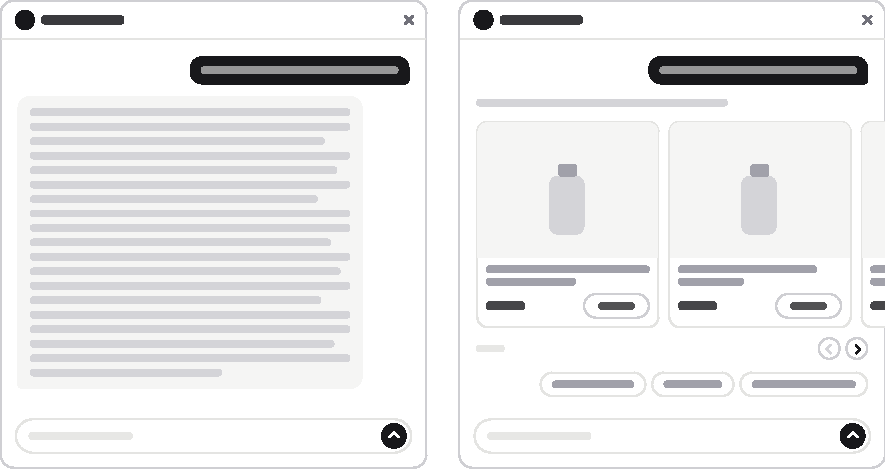
\includegraphics[width=\textwidth]{figure/02-ragioni/confronto.pdf}
	\caption[Confronto tra un assistente testuale e ChatCart]{\emph{Mockup} della risposta alla
	stessa richiesta di un assistente testuale, a sinistra, e di ChatCart, a destra.}
	\label{fig:confronto}
\end{figure}

Il potenziale di un assistente efficace è misurabile. Uno studio sperimentale condotto tra il 2023
e il 2024 su una delle maggiori piattaforme internazionali di commercio
elettronico\textsuperscript{\ref{rif:studio-genai}} ha confrontato sette applicazioni dell’IA
generativa, ciascuna con un gruppo di clienti che la usava e un gruppo di controllo. L’effetto
maggiore è quello dell’assistente che risponde alle domande dei clienti prima dell’acquisto, che ha
aumentato le vendite del 16,3\%. L’aumento deriva da un numero maggiore di clienti che acquistano,
mentre il valore medio del carrello resta invariato. I clienti che traggono più vantaggio
dall’assistente sono quelli che conoscono meno la piattaforma.

Le soluzioni disponibili sul mercato appartengono a cinque tipi, e ciascuno lascia scoperta una
parte del problema:

\begin{itemize}
	\item \textbf{Gli assistenti generici per l’assistenza clienti} risolvono richieste di supporto
	su più canali a partire dai documenti dell’azienda. Conoscono poco il catalogo e rispondono con
	testo, quindi sono adatti alla gestione di un reso più che alla scelta di un prodotto.
	\item \textbf{Gli assistenti alla vendita preconfezionati} si installano nel negozio e
	consigliano prodotti. L’interfaccia, il modello e il comportamento sono decisi dal fornitore e
	restano uguali per tutti i negozi che li adottano.
	\item \textbf{Sidekick}\textsuperscript{\ref{rif:sidekick}}, l’assistente che Shopify integra nel
	pannello di amministrazione, supporta il commerciante nella gestione del negozio e non si
	rivolge a chi acquista.
	\item \textbf{Il \emph{server} MCP del negozio}\textsuperscript{\ref{rif:storefront-mcp}}, che
	Shopify attiva per ogni negozio, espone agli agenti la ricerca nel catalogo, il carrello e le
	condizioni di vendita. È un componente destinato a chi sviluppa un agente, perché fornisce dati
	e operazioni senza un’interfaccia, e la sua ricerca è la stessa per ogni catalogo.
	\item \textbf{\gloss{ucp}{UCP}}\textsuperscript{\ref{rif:ucp}}, uno standard aperto che Shopify
	e Google hanno pubblicato nel gennaio 2026, permette a un agente di scoprire che cosa offre un
	negozio e di completare un acquisto. È pensato per gli assistenti di terze parti, per cui la
	conversazione avviene fuori dal negozio, in un’interfaccia che il marchio non controlla.
\end{itemize}

Nessuna di queste soluzioni soddisfa insieme i tre requisiti a cui i clienti di Halue attribuiscono
più valore, cioè l’identità visiva del marchio, i dati specifici del suo catalogo e un’esperienza
d’acquisto che si svolge interamente nel negozio. Un prodotto preconfezionato deve adattarsi a
tutti i commercianti, e per questo lascia poco spazio alla personalizzazione. Halue costruisce
soluzioni per il singolo cliente, perciò ha scelto di esplorare un assistente su misura basato su
un’\gloss{interfaccia-generativa}{interfaccia generativa}, in cui l’agente risponde con testo
oppure sceglie un componente da una libreria predefinita, come una scheda prodotto, e lo popola in
tempo reale con i dati del negozio. Il marchio conserva il controllo sull’aspetto dei componenti,
e il modello decide soltanto quale mostrare e con quali dati.


% !TeX root = ../../tesi.tex

\section{Il commercio agentico nella visione di Halue}
\label{sec:commercio-agentico}

Il \gloss{commercio-agentico}{commercio agentico} è l’insieme delle esperienze d’acquisto in cui un
agente di intelligenza artificiale accompagna il cliente nella ricerca, nella scelta e
nell’acquisto di un prodotto. Si sta sviluppando in due direzioni:

\begin{itemize}
	\item il negozio si apre ad assistenti generici di terze parti, che lo raggiungono con protocolli
	come MCP e UCP, e il cliente conversa altrove mentre il negozio fornisce catalogo e pagamento;
	\item l’assistente appartiene al marchio e opera all’interno del negozio, con la sua interfaccia
	e con strumenti scritti per il suo catalogo.
\end{itemize}

Le piattaforme promuovono la prima direzione, che un commerciante può adottare senza alcuno
sviluppo dedicato. La seconda richiede un progetto su misura, ed è quella in cui un’azienda come
Halue può offrire un servizio ai propri clienti. ChatCart la esplora.

Prima dello \emph{stage} Halue disponeva già di alcune premesse, cioè i negozi realizzati per
marchi che vendono su più mercati e gli agenti collegati ai dati dei negozi con strumenti propri
(\secref{sec:innovazione}). Non aveva invece esperienza su un assistente rivolto al cliente finale,
che pone problemi diversi da quelli di un agente a uso interno perché deve integrarsi con il tema
del negozio, rispondere in pochi secondi e comportarsi in modo prevedibile con qualsiasi
interlocutore. Lo \emph{stage} aveva lo scopo di costruire questa competenza su un caso
sufficientemente circoscritto da poter essere completato nella durata prevista.

Al termine dello \emph{stage}, il risultato costituisce per l’azienda una base di ricerca e
sviluppo. L’obiettivo dichiarato è arrivare a proporre questo tipo di soluzione ai clienti come
servizio, con tempi e forma ancora da stabilire. Il primo passo è stata la presentazione al
\emph{team} del 9 novembre 2026, l’ultimo giorno di \emph{stage}, articolata in trenta minuti
dedicati al prodotto, quindici alla parte tecnica e quindici alle domande. Le domande hanno
mostrato quali aspetti interessano a chi riprenderà il lavoro, in particolare le scelte di
progettazione, come la gestione dello stato nella sincronizzazione del carrello, e il modo in cui
ho istruito l’agente perché si comportasse come previsto.


% !TeX root = ../../tesi.tex

\section{Obiettivi e vincoli del progetto}
\label{sec:obiettivi}

Mi sono candidato a luglio 2026 e ad agosto ho sostenuto un colloquio conoscitivo con il
\emph{tutor} e con il fondatore. Halue mi ha poi proposto due temi, l’interfaccia generativa e la
gestione del contesto di un agente. Ho scelto il primo e ho proposto di declinarlo in un assistente
che seleziona e popola componenti dell’interfaccia con i dati del negozio.

Il piano organizza il prototipo su due livelli (\figref{fig:livelli}). L’\emph{app layer} è il
\emph{widget} di chat nel negozio e si limita a visualizzare la conversazione e i componenti.
L’\emph{agent layer} è il \emph{backend} che ospita l’agente e conserva lo stato della
conversazione. Per interrogare le API di Shopify l’agente usa il
\gloss{tool-calling}{\emph{tool calling}}, il meccanismo con cui un modello linguistico chiede al
programma che lo ospita di eseguire una funzione e ne riceve il risultato.

\begin{figure}[htbp]
	\centering
	\setstretch{1}
	% L'architettura su due livelli prevista dal piano di lavoro: il widget nel negozio
% (app layer) e il backend che ospita l'agente (agent layer), con i servizi esterni a destra.
% Il disegno è largo quanto il testo (150 mm): si include con \input, senza ridimensionarlo.

\begin{tikzpicture}[
	every node/.style={text=FiguraTesto},
	blocco/.style={draw=FiguraTenue, fill=white, rounded corners=3pt, text width=#1-2mm,
		minimum width=#1, minimum height=13mm, align=center, inner sep=1.5pt,
		font=\fontsize{7.5}{9}\selectfont,
		execute at begin node={\hyphenpenalty=10000\exhyphenpenalty=10000}},
	blocco/.default=32mm,
	etichetta/.style={font=\fontsize{7}{8.5}\selectfont, text=FiguraTenue, inner sep=1pt,
		align=center},
]
	\begin{scope}[on background layer]
		\path[partizione] (0mm, 0mm) rectangle (38mm, -44mm);
		\path[intestazione] (0mm, 0mm) rectangle (38mm, -6mm);
		\node[titolo] at (19mm, -3mm) {\emph{App layer}: negozio};
		\path[partizione] (72mm, 0mm) rectangle (110mm, -44mm);
		\path[intestazione] (72mm, 0mm) rectangle (110mm, -6mm);
		\node[titolo] at (91mm, -3mm) {\emph{Agent layer}: \emph{backend}};
		\path[partizione] (122mm, 0mm) rectangle (150mm, -44mm);
		\path[intestazione] (122mm, 0mm) rectangle (150mm, -6mm);
		\node[titolo] at (136mm, -3mm) {Servizi esterni};
	\end{scope}

	\node[blocco] (widget) at (19mm, -16mm)
		{\voce{\emph{Widget} di chat}{mostra la conversazione}};
	\node[blocco] (componenti) at (19mm, -34mm)
		{\voce{Libreria di componenti}{popolati con i dati del negozio}};
	\node[blocco] (agente) at (91mm, -16mm)
		{\voce{Agente}{sceglie testo o componente, esegue gli strumenti}};
	\node[blocco] (stato) at (91mm, -34mm)
		{\voce{Stato}{storico della conversazione}};
	\node[blocco=24mm] (llm) at (136mm, -16mm) {\voce{Modello linguistico}{genera le risposte}};
	\node[blocco=24mm] (api) at (136mm, -34mm) {\voce{API di Shopify}{catalogo, carrello, ordini}};

	\draw[freccia] ([yshift=3mm]widget.east) -- node[etichetta, above=0.5mm]
		{messaggio del cliente} ([yshift=3mm]agente.west);
	\draw[freccia] ([yshift=-3mm]agente.west) -- node[etichetta, below=0.5mm]
		{testo o componente\\e tre messaggi suggeriti} ([yshift=-3mm]widget.east);
	\draw[freccia] (widget) -- node[etichetta, right=0.5mm] {disegna} (componenti);
	\draw[freccia, {Stealth[length=1.8mm,width=1.4mm]}-{Stealth[length=1.8mm,width=1.4mm]}]
		(agente) -- (stato);
	\draw[freccia, {Stealth[length=1.8mm,width=1.4mm]}-{Stealth[length=1.8mm,width=1.4mm]}]
		(agente.east) -- (llm.west);
	\draw[freccia] (agente.east) ++(0, -3mm) -- ++(6mm, 0) |- (api.west);
\end{tikzpicture}

	\caption[L’architettura su due livelli prevista dal piano di lavoro]{L’architettura su due
	livelli prevista dal piano di lavoro. Il \emph{widget} non contiene logica conversazionale: ogni
	decisione spetta all’agente, che può interrogare più volte modello e API prima di rispondere.}
	\label{fig:livelli}
\end{figure}

Gli obiettivi hanno un identificativo, che uso nel resto della relazione, e tre livelli di
priorità. Gli obiettivi obbligatori (\tabref{tbl:obbligatori}) sono vincolanti e, oltre a
dimostrare la fattibilità dell’approccio, chiedono di misurarne l’efficacia.

Gli obiettivi desiderabili hanno un valore aggiunto riconoscibile, quelli facoltativi un valore
aggiunto non prioritario (\tabref{tbl:desiderabili}). Riprendono tre aspetti che il \emph{tutor}
ha indicato come interessanti per l’azienda: il supporto a più mercati, i temi Hydrogen, in cui il
riuso dei componenti React è più semplice e l’integrazione con il carrello più complessa, e una
ricerca nel catalogo scritta su misura, perché il \emph{tutor} giudicava elementare quella del
\emph{server} MCP di Shopify.

\begin{tabellatesi}{P{0.1}P{0.9}}
	{Gli obiettivi obbligatori del piano di lavoro.}
	{tbl:obbligatori}
	\toprule
	\rowcolor{TabellaIntestazione} \textbf{ID} & \textbf{Obiettivo} \\
	\midrule
	OB1 & \emph{App layer}: \emph{widget} di chat in React e TypeScript integrato nel negozio \\
	OB2 & \emph{Agent layer}: \emph{backend} Node.js con un agente dotato di \emph{tool calling}, in
	grado di interrogare le API di Shopify \\
	OB3 & Risposte in linguaggio naturale (domande generali, sui prodotti, di chiarimento) oppure con
	un componente predefinito, scelto e popolato in base alla conversazione \\
	OB4 & Libreria di almeno due o tre componenti flessibili e tre messaggi suggeriti per ogni
	risposta \\
	OB5 & Raccolta di metriche di coinvolgimento e di conversione sull’uso del \emph{widget} \\
	\bottomrule
\end{tabellatesi}

\begin{tabellatesi}{P{0.1}P{0.2}P{0.7}}
	{Gli obiettivi desiderabili e facoltativi del piano di lavoro.}
	{tbl:desiderabili}
	\toprule
	\rowcolor{TabellaIntestazione} \textbf{ID} & \textbf{Priorità} & \textbf{Obiettivo} \\
	\midrule
	DE1 & desiderabile & Supporto a \gloss{shopify-markets}{Shopify Markets}, la funzione con cui un
	negozio vende in più paesi con lingue e valute diverse \\
	DE2 & desiderabile & Componente per lo stato dell’ordine e il supporto dopo la vendita \\
	FA1 & facoltativo & Prova di fattibilità dell’integrazione su Hydrogen, con il riuso dei
	componenti del \emph{widget} \\
	FA2 & facoltativo & Confronto sperimentale tra la ricerca su misura, il \emph{server} MCP di
	Shopify e un eventuale \emph{server} MCP proprio \\
	\bottomrule
\end{tabellatesi}

Il piano ripartisce 310 ore indicative tra dieci attività (\figref{fig:piano}) e prevede che la
ripartizione sia rifinita con il \emph{tutor} nelle prime settimane. Nel capitolo 3 la confronto
con l’uso effettivo del tempo.

\begin{figure}[htbp]
	\centering
	\setstretch{1}
	% La ripartizione indicativa delle 310 ore prevista dal piano di lavoro, come grafico a torta.
% Le fette seguono l'ordine del piano in senso orario dall'alto: in grigio chiaro le attività che
% precedono il codice, in bordeaux lo sviluppo dei due livelli, in grigio medio quelle successive.
% Il disegno è largo quanto il testo (150 mm): si include con \input, senza ridimensionarlo.

\begin{tikzpicture}[every node/.style={text=FiguraTesto}]
	\def\raggio{22mm}
	\def\inizio{90}
	% ore/colore/lato (1 a destra, -1 a sinistra)/quota dell'etichetta/titolo/dettaglio
	\foreach \ore/\colore/\lato/\quota/\titolo/\dettaglio in {
		20/TabellaIntestazione/1/27/{Studio}/{Shopify e strumenti per agenti},
		20/TabellaIntestazione/1/16/{Analisi dei requisiti}/{e perimetro del progetto},
		20/TabellaIntestazione/1/5/{Progettazione}/{dell’architettura},
		40/TabellaIntestazione/1/-7/{Negozio di sviluppo}/{e accesso ai dati},
		50/FiguraAccento/1/-21/{\emph{Agent layer}}/{sviluppo del \emph{backend}},
		60/FiguraAccento!65/-1/-21/{\emph{App layer}}/{sviluppo del \emph{widget}},
		30/FiguraBordo/-1/-7/{Integrazione}/{del flusso conversazionale},
		30/FiguraBordo/-1/5/{Metriche}/{raccolta dei dati di utilizzo},
		20/FiguraBordo/-1/16/{\emph{Test}}/{flusso utente e casi limite},
		20/FiguraBordo/-1/27/{Documentazione}/{tecnica}} {
		\pgfmathsetmacro\fine{\inizio - \ore/310*360}
		\pgfmathsetmacro\medio{(\inizio + \fine)/2}
		\fill[\colore, draw=white, line width=0.8pt] (0, 0) -- (\inizio:\raggio)
			arc[start angle=\inizio, end angle=\fine, radius=\raggio] -- cycle;
		\draw[FiguraTenue] (\medio:\raggio + 1mm) -- (\lato*\raggio + \lato*10mm, \quota mm)
			-- ++(\lato*3mm, 0);
		\ifnum\lato=1
			\node[anchor=west, align=left, font=\fontsize{7.5}{9}\selectfont]
				at (\raggio + 14mm, \quota mm) {\voce{\titolo, \ore{} ore}{\dettaglio}};
		\else
			\node[anchor=east, align=right, font=\fontsize{7.5}{9}\selectfont]
				at (-\raggio - 14mm, \quota mm) {\voce{\titolo, \ore{} ore}{\dettaglio}};
		\fi
		\global\let\inizio\fine
	}
\end{tikzpicture}

	\caption[La ripartizione delle ore prevista dal piano di lavoro]{La ripartizione delle ore
	prevista dal piano di lavoro, in senso orario dall’alto. In grigio chiaro le attività che
	precedono la scrittura del codice, in bordeaux lo sviluppo dei due livelli, in grigio medio le
	attività che lo completano.}
	\label{fig:piano}
\end{figure}

Per l’azienda il criterio di successo era un prototipo funzionante dall’inizio alla fine su un
negozio di esempio, accompagnato da una valutazione onesta di ciò che funziona e di ciò che non
funziona. Valuto il grado di soddisfacimento di ogni obiettivo nella \secref{sec:soddisfacimento}.

Il progetto aveva i seguenti vincoli:

\begin{itemize}
	\item \textbf{Quantità di lavoro}: da 300 a 320 ore, con una distribuzione al massimo a tempo
	pieno, dal 14 settembre al 9 novembre 2026.
	\item \textbf{Luogo di lavoro}: da remoto, con un giorno a settimana in sede, un allineamento
	quotidiano con il \emph{tutor} e una riunione settimanale di un’ora.
	\item \textbf{Tecnologie}: TypeScript in tutto il progetto. Il piano rimandava alle prime settimane la scelta degli strumenti
	per costruire l’agente e del modello linguistico, che il \emph{tutor} ha lasciato a me.
	\item \textbf{Piattaforma}: prima i temi Liquid, che sono i più diffusi, e Hydrogen soltanto come
	eventuale approfondimento finale.
	\item \textbf{Ambiente}: un unico negozio di sviluppo, senza clienti né traffico reali, con due
	temi installati per le prove. L’ho allestito come un negozio di cosmetica botanica con circa
	quaranta prodotti, perché il comportamento di un assistente dipende dal catalogo su cui opera, e
	varianti, collezioni, confezioni regalo, prodotti esauriti e archiviati lo avvicinano a un caso
	reale.
	\item \textbf{Natura del prodotto}: un prototipo di ricerca e sviluppo, essenziale ma solido,
	senza i requisiti di scala e di costo di un prodotto in produzione.
\end{itemize}


% !TeX root = ../../tesi.tex

\section{Motivazioni e obiettivi personali}
\label{sec:obiettivi-personali}

Da marzo 2026 lavoro in proprio come sviluppatore di negozi Shopify, occupandomi di migrazioni da
altre piattaforme, gestione dei negozi e automazioni. La mia esperienza riguardava però soltanto i
temi Liquid e non lo sviluppo di applicazioni. Tra le proposte di \emph{stage}, quella di Halue
riguardava progetti su Shopify, era la più vicina al mio lavoro e mi offriva ciò che mi mancava:
lo sviluppo di un’applicazione in un’azienda che lavora su questa piattaforma ogni giorno. Per
questo l’ho scelta.

L’idea dell’interfaccia generativa è di Halue. Quando l’azienda me l’ha proposta vi ho riconosciuto
l’esigenza di un mio cliente, che mi aveva parlato di un assistente capace di dare assistenza ai
visitatori del suo negozio e di indirizzarli verso l’acquisto. Il progetto aveva quindi per me un
valore che andava oltre lo \emph{stage}, e questo ha orientato sia la scelta del tema sia la
proposta dei componenti.

Da queste ragioni ho ricavato quattro obiettivi personali (\tabref{tbl:personali}), che valuto
insieme a quelli del piano nella \secref{sec:soddisfacimento}.

\begin{tabellatesi}{P{0.1}P{0.9}}
	{I miei obiettivi personali per lo \emph{stage}.}
	{tbl:personali}
	\toprule
	\rowcolor{TabellaIntestazione} \textbf{ID} & \textbf{Obiettivo} \\
	\midrule
	OP1 & Estendere le mie competenze su Shopify dai temi allo sviluppo di applicazioni \\
	OP2 & Acquisire esperienza nella progettazione di sistemi basati su agenti \\
	OP3 & Ricavare dal progetto conoscenze e soluzioni riutilizzabili nella mia attività
	professionale \\
	OP4 & Gestire in autonomia il lavoro da remoto, dove nessuno segue la mia giornata in modo
	continuo e spetta a me organizzarla, stabilire le priorità e prevedere le pause \\
	\bottomrule
\end{tabellatesi}

% DA CONFERMARE: il cliente resta anonimo finché non autorizza la citazione del nome.


% !TeX root = ../tesi.tex

\iniziocapitoloterzo
\chapter{Progetto e sviluppo di ChatCart}

Racconto lo \emph{stage} come un piccolo progetto a sé stante: il metodo di lavoro, l’analisi, la
progettazione, la realizzazione, le sperimentazioni, la verifica e i risultati.

\section{Metodo di lavoro}

\subsection{Pianificazione e interazione con il \emph{tutor} aziendale}
\label{sec:pianificazione}

Il piano di lavoro assegnava 310 ore indicative a dieci attività, senza distribuirle in un
calendario settimanale. La scelta era coerente con la natura esplorativa del progetto, perché Halue
non
sapeva ancora quale forma avrebbe preso un assistente con interfaccia generativa, e un calendario
dettagliato avrebbe fissato in anticipo decisioni che dipendevano da ciò che avrei scoperto
lavorando. Io e il \emph{tutor} abbiamo quindi tenuto fissi gli obiettivi e stabilito di volta in
volta le attività successive in base allo stato del prototipo. Un procedimento di questo tipo
richiede confronti frequenti, che il piano prevedeva quotidiani e settimanali e che ho adattato al
lavoro prevalentemente da remoto (\tabref{tbl:coordinamento-stage}).

\begin{tabellalunga}{P{0.3}P{0.7}}
	{\textbf{Momento previsto} & \textbf{Svolgimento effettivo}}
	{Le modalità di coordinamento durante lo \emph{stage}.}
	{tbl:coordinamento-stage}
	Allineamento quotidiano con il \emph{team} & Ho partecipato allo \emph{stand-up} mattutino,
	riportando attività concluse, lavoro previsto e impedimenti. \\
	Allineamento quotidiano con il \emph{tutor} & Ho inviato un resoconto scritto di fine giornata
	nel canale Slack dedicato. \\
	Revisione settimanale di un’ora & Io e il \emph{tutor} abbiamo discusso il prototipo, i
	problemi aperti e le attività successive. \\
	Supporto su richiesta & Ho chiesto riunioni aggiuntive quando una scelta bloccava il lavoro;
	in alcuni confronti è intervenuto anche il fondatore. \\
	Presenza in sede & Dopo i primi due giorni in ufficio, sono stato in sede in media un giorno
	a settimana. \\
\end{tabellalunga}

Il lavoro da remoto rendeva il confronto meno immediato che in ufficio, e nelle prime settimane
ponevo le domande al \emph{tutor} troppo tardi, dopo aver dedicato tempo a soluzioni che un
confronto anticipato avrebbe corretto. Ho quindi iniziato a preparare ogni confronto per iscritto,
indicando il risultato atteso, le alternative già provate e le decisioni da prendere insieme. La
forma scritta mi obbligava a definire il problema prima della riunione e lasciava traccia della
decisione presa. Per la sincronizzazione del carrello, per esempio, ho presentato tre possibilità:
specializzare il \emph{widget} per un tema, supportare una famiglia di temi oppure offrire
un’integrazione generica. Da quel confronto è nata la combinazione di adattatori e ripiego
descritta nella \secref{sec:widget}; ciò che ho imparato dalla comunicazione a distanza è oggetto
della \secref{sec:maturazione}.

Il primo passaggio importante è arrivato presto. Nella prima settimana ho studiato l’ecosistema
Shopify e definito il perimetro del progetto; nella seconda ho completato un primo prototipo
funzionante, con cui ho verificato le scelte architetturali concordate con il \emph{tutor}. Alla
fine della terza settimana, dopo circa sette giorni passati a lavorare sul codice, avevo una prima
versione che copriva gli obiettivi obbligatori OB1--OB5. Il \emph{tutor} l’ha valutata
positivamente e, con più di metà dello \emph{stage} ancora da svolgere, abbiamo deciso di dedicare
il tempo restante all’esperienza d’uso e alla sperimentazione, che Halue considerava la parte di
maggior valore del progetto. La prima versione è diventata così una base da mettere alla prova, e
funzionalità e architettura hanno continuato a cambiare fino alle ultime settimane.

Per capire quanto questa decisione abbia modificato la distribuzione del lavoro, ho ripartito a
consuntivo le 304 ore dello \emph{stage} tra le attività del piano, basandomi sulla storia delle
modifiche al codice e sulle date dei documenti di progetto. La \figref{fig:tempi-stage} riporta il
risultato in ore intere e indicative.
% DA CONFERMARE: Edoardo riconosce la ripartizione delle ore almeno per ordine di grandezza?

\begin{figure}[htbp]
	\centering
	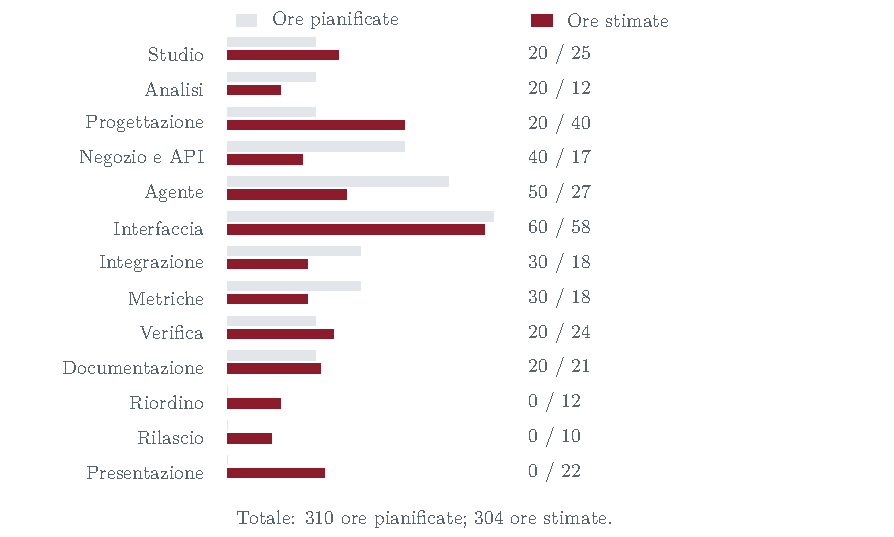
\includegraphics[width=\linewidth]{assets/03-tempi.pdf}
	\caption[Ore pianificate e stimate per attività]{Le ore del piano e la mia stima a consuntivo,
	in valori indicativi. Le ultime tre attività non avevano una voce autonoma nel piano. Le barre
	confrontano quantità di lavoro, senza attribuire al piano un calendario che non prevedeva.}
	\label{fig:tempi-stage}
\end{figure}

La progettazione ha richiesto il doppio delle ore previste, perché vi sono tornato ogni volta che
una prova mostrava un limite della soluzione adottata. La prima realizzazione dell’agente e
dell’accesso al negozio ha richiesto invece circa la metà del tempo previsto, perché il modello
ufficiale di Shopify per le applicazioni forniva già autenticazione, sessioni e integrazione con
l’amministrazione. Lo sviluppo dell’interfaccia si è esteso lungo quasi tutto lo \emph{stage},
comprese le sperimentazioni poi abbandonate, e il tempo risparmiato nelle prime settimane è andato
al riordino del codice, al rilascio e alla presentazione finale al resto del \emph{team}, attività
che il piano non prevedeva come voci autonome. La distribuzione effettiva riflette quindi la
decisione presa alla fine della terza settimana, che ha trasformato un piano pensato per costruire
un prodotto in un percorso di ricerca e sviluppo, in cui provavo ogni soluzione, la valutavo con
il \emph{tutor} e, quando serviva, la rivedevo.

\subsection{Organizzazione del lavoro e tracciamento delle attività}

Illustro come ho organizzato il mio lavoro, svolto in gran parte da remoto: come individuavo le
attività e ne stabilivo le priorità, come ne tenevo traccia e come preparavo le modifiche più estese
prima di realizzarle.

\subsection{Strumenti e assistenti di programmazione}

Presento gli strumenti che ho impiegato per lo sviluppo, la verifica e il rilascio, tra cui gli
assistenti di programmazione basati su modelli linguistici. Di questi descrivo l’uso che ne ho
fatto: la sperimentazione e la validazione rapida delle idee, fino a prototipi funzionanti nell’arco
di una giornata, a cui seguiva l’implementazione definitiva scritta a mano; la stesura dei documenti
di progettazione, per individuare in anticipo i casi limite e i \emph{test} necessari; le attività
di supporto, come la generazione dei dati di prova. Ciò che ho imparato da questo uso lo discuto
nella \secref{sec:maturazione}.

\section{Studio preliminare e analisi}

\subsection{L’ecosistema delle applicazioni Shopify}
\label{sec:ecosistema-applicazioni}

Descrivo la fase iniziale dello \emph{stage}, dedicata allo studio del funzionamento di
un’applicazione Shopify (autenticazione, \emph{app proxy}, estensioni del tema, differenze tra
Storefront API e Admin API) e degli strumenti per la costruzione di agenti. Distinguo le conoscenze
che avevo già acquisito lavorando sui temi Liquid da quelle che ho dovuto costruire per la prima
volta.

\subsection{Un’analisi dei requisiti iterativa}
\label{sec:requisiti}

Motivo la scelta, condivisa con il \emph{tutor}, di non svolgere un’analisi dei requisiti completa
all’inizio del progetto: il lavoro aveva carattere esplorativo, nessun cliente ne dettava i
requisiti, e una specifica fissata a priori sarebbe diventata presto obsoleta. Descrivo il
procedimento che ho seguito: a partire dagli obiettivi del piano ho abbozzato i casi d’uso
principali e ne ho ricavato i requisiti, che ho rivisto a ogni iterazione insieme al prodotto. Un
diagramma mostra i casi d’uso nella loro forma finale e una tabella riporta i requisiti a cui sono
arrivato, raggruppati per area, ciascuno con un identificativo e l’obiettivo del piano da cui
deriva; ne misuro la copertura nella \secref{sec:quantitativi}.

% DA DEFINIRE: prima i casi d'uso iniziali, poi come raggruppare i requisiti (utente, agente, app...). Solo dopo valutare se partire dalla specifica cancellata il 15/10 in chat-cart.

\section{Architettura del sistema}

\subsection{Visione d’insieme}

Illustro l’architettura di ChatCart con un diagramma: il \emph{widget} nel negozio (\emph{app
layer}), il \emph{server} che ospita l’agente (\emph{agent layer}), la \emph{dashboard} del
commerciante e i servizi esterni. Motivo la scelta di uno stile funzionale anziché orientato agli
oggetti, la decisione, su indicazione del \emph{tutor}, di non introdurre astrazioni prima che
fossero necessarie e i \emph{design pattern} che ho adottato quando lo sono diventate.

\subsection{Il contratto tra agente e \emph{widget}}
\label{sec:contratto}

Approfondisco la scelta su cui si regge l’interfaccia generativa: un unico elenco di strumenti,
condiviso tra agente e \emph{widget}, che distingue gli strumenti che leggono i dati del negozio da
quelli che mostrano un componente e chiudono la risposta. Spiego come da questo elenco derivo i tipi
condivisi tra le due parti, così che il \emph{widget} sappia sempre disegnare ciò che l’agente
sceglie.

\section{Realizzazione}

\subsection{L’agente conversazionale}

Descrivo il processo con cui l’agente costruisce una risposta: un ciclo in cui il modello invoca gli
strumenti per consultare il catalogo, finché non seleziona un componente da mostrare. Discuto come
ho ripartito il controllo del comportamento tra le istruzioni al modello e le regole fisse nel
codice, come ho generato i tre messaggi suggeriti e come ho scelto il modello e il livello di
ragionamento, confrontandone velocità e accuratezza. Un diagramma di sequenza segue il percorso di
un messaggio dall’utente alla risposta. Questa parte risponde agli obiettivi OB2 e OB3.

\subsection{Il \emph{widget} e l’integrazione con il tema del negozio}

Presento il \emph{widget}: i componenti (schede prodotto con selezione della variante, schede con le
risposte tratte dalle pagine del negozio, collegamenti alle collezioni), il supporto a più lingue e
valute e, in particolare, la sincronizzazione del carrello con il tema del negozio. Analizzo perché
ogni tema Shopify gestisce il carrello in modo diverso e come ho affrontato il problema con un
\emph{adapter} per ciascun tema e una soluzione di ripiego. Questa parte risponde agli obiettivi
OB1, OB4 e DE1.

\subsection{Metriche di utilizzo e analisi delle conversazioni}

Descrivo gli eventi che il \emph{widget} registra, il \emph{funnel} che la \emph{dashboard} presenta
al commerciante e l’analisi delle conversazioni con Jev, un modello decisionale di TypeSafe AI
uscito durante lo \emph{stage}: a differenza di un modello linguistico generativo, non produce testo
ma restituisce decisioni tipizzate con la loro probabilità. Da qui apro il confronto tra i due tipi
di modello nei compiti decisionali. Questa parte risponde all’obiettivo OB5.

\section{Sperimentazioni e sviluppi futuri}
\label{sec:sperimentazioni}

Dedico questa sezione alle funzionalità che ho sperimentato senza portarle nel prodotto finale,
perché documentano l’orientamento alla ricerca che io e il \emph{tutor} abbiamo dato al progetto
dalla terza settimana: i messaggi di invito che comparivano prima dell’apertura della chat, i tre
tentativi di adattare l’aspetto del \emph{widget} al tema del negozio, l’impiego di Jev nella scelta
dei componenti, il pannello a tutto schermo su \emph{desktop}. Per ciascuna espongo l’ipotesi di
partenza, l’esito che ho osservato e le ragioni per cui io e il \emph{tutor} abbiamo deciso di non
inserirla nel prodotto consegnato. Da queste prove ricavo infine le strade lungo cui ChatCart
potrebbe evolvere in futuro.

% DA CONFERMARE: quali strade di evoluzione indicare.

\section{Verifica e validazione}
\label{sec:verifica}

Illustro la mia strategia di verifica: \emph{test} automatici concentrati sui punti in cui ChatCart
interagisce con sistemi esterni che non controllo, eseguiti su una base di dati reale e senza
simulare i moduli interni, e le ragioni di questa scelta. Discuto i limiti dei \emph{test}
tradizionali applicati a un agente che non risponde mai due volte nello stesso modo. Concludo con la
validazione svolta insieme al \emph{tutor} e con il rilascio dell’applicazione \emph{online}.

\section{Risultati}

\subsection{Il prodotto dal punto di vista dell’utente}

Presento ChatCart dal punto di vista di chi lo utilizza, attraverso una sequenza di schermate: un
cliente che cerca un prodotto, lo confronta con altri, lo aggiunge al carrello e raggiunge il
pagamento; poi il commerciante che consulta il \emph{funnel} e le conversazioni nella
\emph{dashboard}. Dichiaro inoltre i limiti noti del prototipo.

\subsection{Risultati quantitativi}
\label{sec:quantitativi}

Riporto in tabelle i dati quantitativi del progetto: la copertura dei requisiti definiti nella
\secref{sec:requisiti}, la copertura dei \emph{test} con le scelte che la motivano, le righe di
codice per ciascuna parte dell’applicazione e i documenti che ho consegnato al \emph{team}.

\finecapitoloterzo

% !TeX root = ../tesi.tex

\chapter{Valutazione retrospettiva}

Ripercorro lo \emph{stage} a posteriori: in che misura ho raggiunto gli obiettivi, che cosa ho
imparato e quanto la formazione universitaria mi abbia preparato al lavoro che ho svolto.

% !TeX root = ../../tesi.tex

\section{Soddisfacimento degli obiettivi}
\label{sec:soddisfacimento}

Valuto, sulla base di dati di fatto, il grado di soddisfacimento degli obiettivi presentati nella
\secref{sec:obiettivi} e nella \secref{sec:obiettivi-personali}: una tabella riporta ciascun
obiettivo del piano, da OB1 a FA2, e ciascuno dei miei obiettivi personali, con il relativo stato e
l’evidenza che lo documenta. Valuto allo stesso modo i prodotti attesi: quelli elencati nel piano di
lavoro e la presentazione formale al \emph{team} che il \emph{tutor} mi ha chiesto a fine
\emph{stage}. Discuto gli scostamenti, come gli obiettivi che io e il \emph{tutor} abbiamo scartato
e i limiti delle metriche raccolte.


% !TeX root = ../../tesi.tex

\section{Maturazione professionale}
\label{sec:maturazione}

Descrivo la mia maturazione professionale in termini di conoscenze, come l’ecosistema delle
applicazioni Shopify e la costruzione di agenti, e di abilità, come il lavoro da remoto, la
comunicazione con il \emph{tutor}, la gestione del tempo e la capacità di stabilire cosa escludere
dal progetto. Rifletto inoltre su ciò che ho appreso dall’uso dell’intelligenza artificiale nella
programmazione, il tema su cui si è concentrato l’incontro conclusivo con il fondatore.


% !TeX root = ../../tesi.tex

\section{Formazione universitaria e lavoro}

Confronto le competenze che lo \emph{stage} mi ha richiesto con quelle che ho acquisito nel corso di
studi. Individuo quelle che si sono rivelate utili e le lacune che sono emerse, come la
progettazione di agenti e la verifica di sistemi dal comportamento non deterministico, sia rispetto
allo \emph{stage} sia rispetto all’idea che ho del mondo del lavoro.



% !TeX root = ../tesi.tex

\capitolononnumerato{Acronimi e abbreviazioni}

Elenco in ordine alfabetico gli acronimi e le abbreviazioni introdotti nel capitolo 1. Quando
presente, il collegamento rimanda all’approfondimento nel glossario.

\rimandoglossario{adr}{\textbf{ADR}}: \emph{Architecture Decision Record}.

\rimandoglossario{api}{\textbf{API}}: \emph{Application Programming Interface}.

\textbf{AWS}: Amazon Web Services.

\rimandoglossario{b2b}{\textbf{B2B}}: \emph{Business-to-Business}.

\rimandoglossario{b2c}{\textbf{B2C}}: \emph{Business-to-Consumer}.

\textbf{CMS}: \emph{Content Management System}.

\rimandoglossario{crm}{\textbf{CRM}}: \emph{Customer Relationship Management}.

\rimandoglossario{erp}{\textbf{ERP}}: \emph{Enterprise Resource Planning}.

\textbf{IA}: intelligenza artificiale.

\rimandoglossario{ipaas}{\textbf{iPaaS}}: \emph{Integration Platform as a Service}.

\rimandoglossario{llm}{\textbf{LLM}}: \emph{Large Language Model}.

\rimandoglossario{mcp}{\textbf{MCP}}: \emph{Model Context Protocol}.

\rimandoglossario{sal}{\textbf{SAL}}: stato di avanzamento dei lavori.

\rimandoglossario{semver}{\textbf{SemVer}}: \emph{Semantic Versioning}.

\rimandoglossario{ucp}{\textbf{UCP}}: \emph{Universal Commerce Protocol}.

\textbf{UI}: \emph{User Interface}.

\textbf{UX}: \emph{User Experience}.

% !TeX root = ../tesi.tex

\capitolononnumerato{Glossario}

Raccolgo in ordine alfabetico i termini tecnici introdotti nel testo. Alla prima occorrenza nel
corpo della relazione, il termine e il pedice G rimandano alla voce corrispondente.

\begin{description}
\voceglossario{adr}{ADR}{
        Documento che registra una decisione di architettura: il contesto in cui nasce, le
	alternative considerate, la scelta e le sue conseguenze. Conserva le motivazioni della scelta anche
	quando cambia chi lavora al progetto.
}

\voceglossario{api}{API}{
        Interfaccia con cui un programma rende disponibili dati o operazioni ad altri programmi,
	secondo un contratto definito. In Shopify, la Admin API permette di amministrare il negozio; la
	Storefront API espone le funzioni rivolte all’esperienza d’acquisto.
}

\voceglossario{b2b}{B2B}{
        Modello commerciale in cui un’azienda vende prodotti o servizi ad altre aziende. Nel
	commercio elettronico può richiedere cataloghi, listini e condizioni di acquisto diversi per
	ciascun cliente.
}

\voceglossario{b2c}{B2C}{
        Modello commerciale in cui un’azienda vende prodotti o servizi al consumatore finale. È il
	contesto dell’interfaccia conversazionale di ChatCart, rivolta a chi acquista nel negozio.
}

\voceglossario{crm}{CRM}{
        Insieme di pratiche e sistemi per gestire le relazioni di un’azienda con i propri clienti.
	Un sistema CRM raccoglie, per esempio, contatti, interazioni commerciali e richieste di assistenza.
}

\voceglossario{design-system}{\emph{Design system}}{
        Insieme coerente di principi, regole visive e componenti riusabili per progettare
	un’interfaccia. Comprende elementi come colori, tipografia, spaziature e comportamenti dei
	componenti, così da mantenere riconoscibile l’identità del prodotto o del marchio.
}

\voceglossario{e-commerce}{\emph{E-commerce}}{
        Commercio di prodotti o servizi attraverso canali digitali. Un negozio elettronico comprende
	il catalogo, la selezione dei prodotti, il carrello e il pagamento, oltre ai collegamenti con i
	sistemi che gestiscono ordini e logistica.
}

\voceglossario{erp}{ERP}{
        Sistema gestionale che integra dati e processi di diverse aree aziendali, come
	amministrazione, acquisti, magazzino e vendite. Il collegamento con il negozio permette, per
	esempio, di sincronizzare ordini e disponibilità dei prodotti.
}

\voceglossario{founder-senior-consultant}{\emph{Founder \& Senior Consultant}}{
        Ruolo che unisce la fondazione dell’azienda all’attività di consulenza esperta. In Halue lo
	ricopre Valentino Baraldo.
}

\voceglossario{graphql}{GraphQL}{
        Linguaggio di interrogazione per API e insieme di regole per eseguire le richieste su uno
	schema di dati tipizzato. Il programma che invia la richiesta specifica i campi di cui ha bisogno;
	Shopify lo adotta per la Admin API e la Storefront API.
}

\voceglossario{headless}{\emph{Headless}}{
        Architettura che separa la gestione dei dati e delle funzioni applicative dall’interfaccia
	che li presenta. In un negozio di questo tipo l’interfaccia è un’applicazione autonoma che comunica
	con la piattaforma commerciale tramite API; in un CMS la stessa separazione riguarda i contenuti e
	la loro presentazione.
}

\voceglossario{hydrogen}{Hydrogen}{
        \emph{Framework} di Shopify basato su React per costruire interfacce di negozi
	\emph{headless}. Offre strumenti e componenti per accedere ai dati del negozio tramite la
	Storefront API; Oxygen è il servizio di Shopify che può ospitare queste applicazioni.
}

\voceglossario{ipaas}{iPaaS}{
        Piattaforma erogata come servizio per collegare applicazioni e sistemi diversi. Offre
	connettori e strumenti per trasformare e trasferire i dati, riducendo la necessità di costruire
	un’integrazione distinta per ogni coppia di sistemi.
}

\voceglossario{junior-developer}{\emph{Junior Developer}}{
        Sviluppatore all’inizio del proprio percorso professionale, che realizza e verifica
	funzionalità con il supporto di colleghi più esperti.
}

\voceglossario{liquid}{Liquid}{
        Linguaggio di \emph{template} usato nei temi Shopify. Permette di combinare la struttura
	delle pagine con i dati del negozio, attraverso variabili, condizioni e cicli; la piattaforma
	elabora i modelli e genera le pagine da inviare al navigatore.
}

\voceglossario{llm}{LLM}{
        Modello linguistico di grandi dimensioni, addestrato su ampie raccolte di dati per elaborare
	e generare testo. In un agente può selezionare strumenti esterni di cui l’applicazione esegue le
	operazioni; il collegamento a questi strumenti gli permette di usare dati aggiornati che non fanno
	parte del suo addestramento.
}

\voceglossario{mcp}{MCP}{
        Protocollo aperto che standardizza la comunicazione tra applicazioni basate su modelli
	linguistici e servizi esterni. Un \emph{server} MCP può esporre strumenti, risorse e istruzioni; è
	l’applicazione che ospita il modello a gestire il collegamento e l’esecuzione delle richieste.
}

\voceglossario{project-management-assistant}{\emph{Project Management Assistant}}{
        Figura che supporta la gestione dei progetti, contribuendo all’organizzazione delle
	attività, all’aggiornamento della documentazione e al monitoraggio delle scadenze.
}

\voceglossario{project-service-manager}{\emph{Project/service manager}}{
        Responsabilità operativa di gestione di un progetto o di un servizio continuativo. Nel
	metodo di Halue cura la pianificazione delle attività e la capacità disponibile del gruppo di
	lavoro.
}

\voceglossario{pull-request}{\emph{Pull request}}{
        Proposta di integrare un insieme di modifiche da un \emph{branch} a un altro in un sistema
	di versionamento. Raccoglie le differenze nel codice, la discussione di revisione e gli esiti dei
	controlli automatici prima dell’integrazione.
}

\voceglossario{sal}{SAL}{
        Stato di avanzamento dei lavori. Nel contesto descritto indica un rapporto periodico che
	riassume il progresso del progetto, le scadenze, i rischi e i punti aperti, per condividere la
	situazione con le persone coinvolte.
}

\voceglossario{scrum}{Scrum}{
        \emph{Framework} per affrontare problemi complessi attraverso cicli brevi di lavoro,
	chiamati \emph{sprint}, e un confronto regolare sui risultati. Prevede responsabilità, eventi e
	artefatti definiti; nella \secref{sec:organizzazione-halue} distinguo questo riferimento
	dall’adattamento che Halue ne fa per il lavoro su commessa.
}

\voceglossario{semver}{SemVer}{
        Convenzione di versionamento semantico che esprime una versione nella forma
	\texttt{MAJOR.MINOR.PATCH}. Rispetto all’API pubblica dichiarata, il primo numero cambia per
	modifiche incompatibili, il secondo per nuove funzionalità compatibili e il terzo per correzioni
	compatibili.
}

\voceglossario{senior-project-manager}{\emph{Senior Project Manager}}{
        Figura con esperienza nella gestione dei progetti, responsabile del coordinamento di
	pianificazione, risorse e avanzamento delle attività.
}

\voceglossario{senior-software-engineer}{\emph{Senior Software Engineer}}{
        Professionista dello sviluppo del \emph{software} con esperienza consolidata, che affronta
	problemi progettuali complessi e contribuisce alle scelte tecniche e alla revisione del codice.
}

\voceglossario{skill}{\emph{Skill}}{
        Insieme riusabile di istruzioni e, quando necessari, risorse o strumenti, che guida un
	assistente basato su IA in un’attività specifica. Serve a rendere esplicito un procedimento, ma non
	garantisce da solo la correttezza dell’esecuzione.
}

\voceglossario{societa-benefit}{Società Benefit}{
        Società che affianca allo scopo di lucro una o più finalità di beneficio comune indicate
	nello statuto. La disciplina italiana richiede una gestione che bilanci questi obiettivi e una
	relazione annuale sull’impatto prodotto; la qualifica non coincide con una certificazione privata
	di sostenibilità.
}

\voceglossario{software-engineer}{\emph{Software Engineer}}{
        Professionista che applica metodi di ingegneria del \emph{software} alla progettazione,
	realizzazione, verifica e manutenzione di sistemi \emph{software}.
}

\voceglossario{solution-technical-architect}{\emph{Solution \& Technical Architect}}{
        Figura che traduce le esigenze applicative in una soluzione tecnica, definendo
	l’architettura del sistema, le tecnologie e le integrazioni tra componenti.
}

\voceglossario{sprint}{\emph{Sprint}}{
        Ciclo di lavoro di durata fissa, non superiore a un mese nel riferimento Scrum, durante il
	quale il gruppo persegue un obiettivo concordato. La revisione dei risultati e la retrospettiva
	permettono di adattare il prodotto e il modo di lavorare al ciclo successivo.
}

\voceglossario{staging}{\emph{Staging}}{
        Ambiente separato dalla produzione in cui collaudare una versione dell’applicazione prima di
	renderla disponibile agli utenti. Riproduce le condizioni di esercizio per quanto necessario alla
	verifica, senza coincidere con il servizio effettivamente usato dai clienti.
}

\voceglossario{storefront}{\emph{Storefront}}{
        Interfaccia di un negozio digitale rivolta al cliente, attraverso cui consultare il
	catalogo, selezionare prodotti e avviare l’acquisto. In Shopify può basarsi sui temi della
	piattaforma oppure su un’applicazione separata con architettura \emph{headless}.
}

\voceglossario{story-point}{\emph{Story point}}{
        Unità di stima relativa che un gruppo usa per confrontare le attività in termini di
	complessità, impegno e incertezza. Non corrisponde a un numero fisso di ore e acquista significato
	rispetto alle stime dello stesso gruppo; la scala di Fibonacci è una possibile convenzione, non un
	obbligo di Scrum.
}

\voceglossario{team-lead}{\emph{Team lead}}{
        Responsabilità di guida tecnica di un gruppo di lavoro. In Halue comprende l’analisi
	funzionale, le stime per il cliente e il coordinamento tecnico degli sviluppatori.
}

\voceglossario{ticket}{\emph{Ticket}}{
        Unità di lavoro registrata in un sistema di tracciamento, con un identificativo, una
	descrizione e uno stato. Può rappresentare una funzionalità, una modifica o un difetto, e
	raccogliere stime, discussioni e collegamenti alle modifiche del codice.
}

\voceglossario{ucp}{UCP}{
        Protocollo aperto per rendere interoperabili i servizi commerciali e gli agenti che operano
	per conto dell’utente. Definisce modalità condivise per scoprire le capacità di un negozio e
	interagire con le fasi dell’acquisto; riguarda il dominio commerciale, mentre MCP offre un
	meccanismo generale per collegare applicazioni e strumenti.
}

\voceglossario{ux-ui-digital-consultant}{\emph{UX/UI Digital Consultant}}{
        Consulente che progetta l’esperienza utente e l’interfaccia di un prodotto digitale,
	considerando percorsi d’uso, struttura delle informazioni e aspetto visivo.
}
\end{description}

% !TeX root = ../tesi.tex

\capitolononnumerato{Riferimenti}
\label{cap:riferimenti}

\begin{itemize}
        \item Halue S.r.l., sito istituzionale, \url{https://halue.com/it}, pagine «Chi siamo»,
	«Approccio» e «Progetti», consultate il 4 novembre 2026.
\end{itemize}


\end{document}
